\documentclass[conference]{IEEEtran}

% use bibliography

\IEEEoverridecommandlockouts
% The preceding line is only needed to identify funding in the first footnote. If that is unneeded, please comment it out.
\usepackage{cite}
\usepackage[numbers]{natbib}
\usepackage{graphicx}
\usepackage{textcomp}
\usepackage{xcolor}
\usepackage{algorithm}
\usepackage{algpseudocode}
\usepackage{amsmath}
\usepackage{amssymb}
\usepackage{amsfonts}
\usepackage{hyperref}
\usepackage{tabularx}
\usepackage{subfigure}
\usepackage{subcaption}
% make the reference in the format [1,2]
% define the format of the reference

%\def\BibTeX{{\rm B\kern-.05em{\sc i\kern-.025em b}\kern-.08em
%    T\kern-.1667em\lower.7ex\hbox{E}\kern-.125emX}}
\begin{document}

\title{LLM Driven Ontology-based methods for Renovation Hazards Evaluation\\
{\footnotesize \textsuperscript{*}Note: Sub-titles are not captured in Xplore and
should not be used}


\thanks{Identify applicable funding agency here. If none, delete this.}
}

\author{\IEEEauthorblockN{1\textsuperscript{st} Zhang Chi}
\IEEEauthorblockA{\textit{dept. name of organization (of Aff.)} \\
\textit{name of organization (of Aff.)}\\
City, Country \\
email address or ORCID}
}

\maketitle

\begin{abstract}
This document is a model and instructions for \LaTeX.
This and the IEEEtran.cls file define the components of your paper [title, text, heads, etc.]. *CRITICAL: Do Not Use Symbols, Special Characters, Footnotes, 
or Math in Paper Title or Abstract.
\end{abstract}

% \begin{IEEEkeywords}

% \end{IEEEkeywords}

\section{Introduction}
\label{sec:introduction}
\subsection*{Background}
\label{sec:background}
With the development of urbanization and population growth, 
the necessity for building renovation is becoming increasingly important, especially in areas with loads of existing buildings, such as Europe \cite[]{jensen2015value}.
% point out the risk of building renovation
Building renovation involves a variety of risks and hazards that can threaten the safety of workers and occupants.
According to the European Union and the UK report, 
the construction industry's average rate of injuries and fatalities is four times higher than in other sectors \cite[]{estudillo2024role,britain2001health}. 
In the US, the fatalities of construction workers account for 20\% of the total fatalities in the workplace \cite[]{kim2016integrating}.

% point out the difficulty of safety management and regulation, and necessity of build an ontology to organize the knowledge for renovatin
% To reduce the risks and hazards in building renovation, risk and safety assessment is critical \cite[]{xing2019ontology}.
% However, in reality, 
% it is difficult to manually and globally evaluate the safety risks, 
% especially when engineers lack professional knowledge and experience \cite[text]{xing2019ontology}. There are two main reasons for this difficulty.
% Firstly, the data related to risk and safety are scattered in different sources, such as regulations, standards, and guidelines \cite[]{xing2019ontology,ding2013development}.
% The unstractured data make it difficult to be used for risk and safety assessment. 
% Secondly the risk identification and evaluation are data-intensive tasks, which is quite time-consuming and labor-intensive \cite[]{qi2023bim,fang2020knowledge}.
% For human beings, it is difficult to process a large amount of data and extract the useful information from them \cite[]{fang2020knowledge,zhang2017integrating}.
% % introduce the ontology-based methods for safety management
%automatically risk and safety assessment methods are proposed \cite[]{xing2019ontology,doukari2023bim,amorocho2021reno,qi2023bim,zhou2023bim}.
To overcome the challenges of safety management in building renovation, automatically risk and safety assessment systems are gaining more and more attention \cite[]{xing2019ontology,doukari2023bim,amorocho2021reno,qi2023bim,zhou2023bim}. 
Ontology is defined by Gruber as a formal, explicit specification of a shared conceptualization \cite[]{gruber1995toward}. 
The ontology provides at least two benefits for automatic safety management system development. Firstly, ontology can organize the knowledge in a structured way, which can help to improve the efficiency of knowledge management \cite[]{zhang2015ontology}. 
Secondly, it converts knowledge into a machine-readable format \cite[]{donini1996reasoning}, which makes it possible to automatically identify and evaluate risks and hazards from given information sources.
As a result, the ontology-based safety management systems have been widely applied to the Architectural, Engineering, and Construction (AEC) industry \cite[]{zhong2015ontological,zhang2015ontology,wang2011ontology,guo2017ontology,xing2019ontology,gao2022knowledge}.

The ontology-based safety management system development process includes three steps: ontology construction, knowledge extraction, knowledge reasoning, and query \cite[]{doukari2024ontology,fang2020knowledge,wang2011ontology}. 
Firstly, the ontology is constructed by domain experts. It includes concepts, properties, and relationships. The ontology hierarchically organizes knowledge and specializes in the relationships between concepts. 
Secondly, entities and relationships are extracted from information sources such as documents, images, and videos. 
Finally, the knowledge inference is conducted to provide the risk and safety assessment results \cite[]{doukari2024ontology,fang2020knowledge}.

% introduce the combination of bim and ontology
%Recently, the combination of Building Information Modeling (BIM) and ontology has been proposed to improve the safety management system in building renovation \cite[]{qi2023bim,zhou2023bim,shen2022safety}. 
The combination of Building Information Modeling (BIM) and ontology has become a trend in the safety management system development \cite[]{qi2023bim,zhou2023bim,shen2022safety}.
The BIM is a digital representation of the physical and functional characteristics of a building \cite[]{qi2023bim}.
Compared with 2D information, BIM provides more dynamic and comprehensive 3D information, which can help to improve the accuracy of risk and safety assessment \cite[]{ding2016construction}. 

%Another development direction is combination of applying multi-modal methods with ontology-based methods to improve the accuracy and efficiency of safety management system. 
With the development of computer vision and natural language processing, 
Combining artificial intelligence and ontology-based methods that take advantage of multi-modal information is another way to improve the safety management system.
Artificial intelligence can help automatically extract entities and relationships from documents and images, improving the efficiency and accuracy of information extraction and query \cite[]{zhong2020ontology,zhang2022automatic}.

%Currrent multi-modal methods are usually used for information extraction \cite[]{zhong2020ontology,zhang2022automatic}. 
\subsection*{Research Gap}
\label{sec:research_gap}
Reviewing the literature, we have identified two research gaps in developing building renovation safety management systems.

Firstly, although the application of BIM and multi-modal methods improve the efficiency and accuracy of information extraction and query, 
the ontology construction process is still manually conducted by domain experts through literature review, interviews, workshops, etc.,
which is time-consuming and labor-intensive \cite[]{doukari2024ontology,amorocho2021reno,shen2022safety,xing2019ontology,zhou2023bim}.

Secondly, the limitation of existing ontology construction and reasoning tools and platforms is another research gap.
Most ontology-based safety management systems research is developed on Protégé, a widely used ontology construction and reasoning platform. 
The knowledge reasoning engine on Protégé, such as Jena and Pellet, is user-friendly and widely used to discover the implicit knowledge from the ontology \cite[]{amorocho2021reno,doukari2024ontology,doukari2023bim}.   
But Protégé stores ontology in OWL files, which stores ontology in XML format \cite[]{mohan2011constructing}.  
XML's verbose and complex format makes integrating with other tools and platforms challenging.   

Based on the research gaps, we propose a novel method using a large language model (LLM) to extract entities and relationships from documents and images automatically,
to construct an ontology-based safety management system for building renovation.
We also developed a tool to convert the ontology from OWL to JSON format and store it in Neo4J, a graph database that can store and query data more efficiently.
Many programming languages and tools provide APIs to access Neo4J, which makes the safety management system more flexible and scalable.

In summary, the contributions of this paper are as follows:
\begin{enumerate}
    \item We develop a tool to convert OWL format to JSON and store it in Neo4J.
    \item We propose a framework to construct ontology for building renovation safety management systems using LLM.
    \item We design an ontology-based automatic risk identification system with BIM using LLM.
\end{enumerate}
% Firstly, although the application of BIM and multi-modal methods improve the efficiency and accuracy of information extraction and query, the ontology construction process is still a bottleneck in the safety management system development.
% Usually the construction of ontology is through literature review, interviews, and workshops, which is time-consuming and labor-intensive \cite[]{doukari2024ontology,amorocho2021reno,shen2022safety,xing2019ontology,zhou2023bim}. 

% We identify a research gap in the ontology construction process, which is the lack of a systematic and automatic method to construct ontology for building renovation safety management system. 
% We propose a novel method using large language model (LLM) to automatically extract entities and relationships from documents and images, 
% to construct ontology-based safety management system for building renovation. 

% Another research gap is that limitation of existing ontology construction and reasoning tools and platforms. Most research of ontology-based safety management system 
% are developed on Protégé, which is a widely used ontology construction and reasoning platform. Protégé stores ontology in OWL format, which stores ontology in XML format \cite[]{mohan2011constructing}.
% The knowledge reasoning engine on Protégé, such as Jena and Pellet, is user-friendly and widely used to discover the implicit knowledge from the ontology \cite[]{amorocho2021reno,doukari2024ontology,doukari2023bim}.
% The risk and safety assessment is conducted by querying on inference eigine on Protégé given the triplets extracted information source like bim, document or images \cite[]{zhong2020ontology,amorocho2021reno,xiong2019onsite}.
% Although Protégé is widely used, the verbose and complex format of OWL makes it difficult to be integrated with other tools and platforms. 
% To integrate the ontology with LLM, we convert the ontology from OWL to JSON format and store it in Neo4J, 
% which is a graph database that can store and query data in a more efficient way. 
% Many programming languages and tools provide APIs to access Neo4J, which make the safety management system more flexible and scalable.

\subsection*{Research Scope}
\label{sec:research_scope}
The research scope of this paper is the construction of ontology for building renovation of a safety management system. 
We only focus on risk identification and evaluation in building renovation and do not consider other aspects of the safety management system, such as safety training and safety culture.
We also do not consider risk and safety assessments at other stages of the building life cycle, such as design and construction.

% Although many scholars have been working on the construction process and operation performance, the renovation of buildings is still a negelcted area \cite{doukari2024ontology}.





% how to make it directly append after the introduction, not a new page

\section{Related Work}
\label{sec:related_work}  
\subsection*{Building Renovation Activities}
Accoridng to the definition of the Global Building Performance Network (GBPN) \cite[]{shnapp2013deep},  
renovation activities is a process asscociated mainly with building envelope of improving existing images or modernizing buildings in a good condition \cite[]{amorocho2021reno}.
Many researchers have mentioned the difficulty and obstacle to implement safety management in renovation activities \cite[]{doukari2024ontology,amorocho2021reno}.
% The first challenge is the complexity and uncertainty of the renovation activities \cite[]{european2020renovation}. 
% \cite{singh2014investigation,salvalai2017deep} pointed out the due to the effects of building residents, 
% the safety management faces many uncertainties and risks. 
% Some protection measures may have to been taken for a long time for the safety of residents such as the prevention of dust and noise \cite[]{salvalai2017deep}.
\cite{singh2014investigation,salvalai2017deep} pointed out the complexity and uncertainty of the renovation activities. 
For example, the effects of building residents may cause many uncertainties and risks, some protection measures may have to been taken for a long time for the safety of residents such as the prevention of dust and noise \cite[]{salvalai2017deep}.

\cite{doukari2024ontology,amorocho2021reno} stressed that for the safety management in renovation activities, a comprehensive knowledge of building components, construction methods, safety regulations and safety measures is required.
 Current guidelines and instructions \cite[]{xu2023comparative,arena2016construction} are gathered from common construction activities, which are not enough to support the safety management in renovation activities \cite[]{doukari2024ontology}.
As a results, the fragmentation of knowledge and lacks of professional personnel for safety management in renovation activities 
may lead to the increase of accidents and high safety management costs \cite[]{buser2019interactive,rodger2019integration}.

Ontology, as a formal and explicit specification of a shared conceptualization \cite[]{gruber1995toward}, 
can be used to organize and represent the knowledge of building renovation activities, boosting the safety management in renovation activities \cite[]{doukari2024ontology,amorocho2021reno}.

\subsection*{Ontology-based Risk Management System}
Ontology-based safety management system has been widely applied to Architectural, Engineering and Construction (AEC) industry.
\cite{zhong2015ontological} utilized ontology for construction regulation and rules to support to ensure the compliance of building codes, regulations and client requirements. \cite{zhang2015ontology,wang2011ontology} proposed an ontology-based job hazard analysis system to generate job hazard analysis reports including potential hazards and related regulations. 
\cite{guo2017ontology} developed an ontology for active fall protection system to reduce the risk of fall accidents in construction sites. 
SRI-Onto \cite[]{xing2019ontology} is an ontology-based system composed of three components: fact base management, rule base management and case based management. Applying SPARQL query language, 
SRI-Onto can identify related risks and provide corresponding rules and cases to support decision-making. 
\cite{gao2022knowledge} introduced ontology-based methods for health and safety management in all stages of construction projects. 

In recent years, ontology-based safety management system has been applied to \textbf{building renovation activities}. 
\cite{amorocho2021reno} build ontology via literature review, interviews with experts and workshops to support the safety management in renovation activities. 
\cite{doukari2024ontology} integrate build ontology on Protégé and integrate it with BIM to support the safety management in renovation activities. 

Although the various ontology-based safety management systems have been proposed, they share common components and workflows.
Firstly, the ontology is built by domain experts and knowledge engineers manually. Scholars and experts define the concepts, properties and relationships of the ontology.
Secondly, the ontology is always built on Protégé using semantic web rule language (SWRL) and performs knowledge reasoning via knowledge reasoning engines like Jena or JESS.   
Lastly, the knowledge inference is performed to support safety management given elements extracted from information sources like BIM, CAD, and documents.  

\subsection*{Multi-modal methods in Building Evaluation}
To support the safety management in renovation activities, multi-modal methods have been proposed to extract knowledge from different sources.
\subsubsection*{BIM} 
More and more researchers have realized the value of Building Information Modeling (BIM) in safety management in construction projects \cite[]{ding2016construction}.
And we ovserve a trend that combining BIM with ontology to support safety management in construction projects. 
\cite{shen2022bim} applied bim for safety management in prefabricated building construction. Applying programming detection algorithm implemented in JAVA, a mapping between 
owl file and BIM model is established, and then knowledge inference is performed to generate risk identification and related rules \cite[]{shen2022bim}. 
\cite{zhou2023bim} extract context information from BIM and stroe it into relational database (RDB), by applying mapping between 
tables in RDB with ontology, the information is converted to triplets and then knowledge inference is performed to support safety management in construction projects \cite[]{zhou2023bim}.
\cite{qi2023bim} applying BIM and ontology for conflict detection and resolving for manufacturing design and assembly for prefabricated buildings. 
Unlike other method directly extract semantic information from BIM, \cite{xu2022ontology} use the data analysis and simulation results to establish mapping between BIM and ontology for damage assessment in construction projects.

Inspired by the success of BIM and ontology in safety management in construction projects, in recent research of safety management in renovation activities, BIM and ontology are also combined to support risk identification and mitigation \cite[]{doukari2024ontology}.

\subsubsection*{Natural Language Processing}
Similar to BIM, natural language processing (NLP) has also been applied for knowledge inference in ontology-based safety management in construction projects.
Traditional rule-based information extraction are rigid and hard to generalize, while deep learning-based NLP methods are more flexible and generalizable for information 
extraction and integration \cite[]{zhang2021semantic}. \cite{zhang2021semantic} leverages transformer-based methods to extract semantic representation from BIM and regulation documents for compliance checks, 
which reaches an accuracy of 80\%. Combined with ontology, NLP based methods are able to help mapping the components of BIM with concepts in ontology for knowledge inference \cite[]{ding2016construction,zhou2021semantic}. 
\cite{shen2022bim} mainly use NLP to efficient query risk information in interested regions from BIM in onlogy-based safety management system, 
simplifying the process to filter inferred knowledge from report.

\subsubsection*{Images}
The advancement of computer vision has enabled the extraction of semantic information from images to support safety management in construction projects.
In construction activities, especially during the construction phase, the images data provide ability to dynamically monitor the construction process and identify potential risks.
\cite{zhang2022automatic} constructed scene graphs from images via transformer-based neural networks and applying C-Bert to achieve automatical regulation compliance checks.
\cite{zhong2020ontology} develops a HowNet-based network to extract semantic relation of objects in images and establish a semantic-based database for 
risk query and knowledge inference. 
The method of \cite{fang2020knowledge} extract objects and their spatial relations from images by ResNet. Compared with risk identification system integrating images, \cite{fang2020knowledge} used similar methods, but directly store the triplets of ontology in graph database for better relation representations and efficient query. 
\cite{lee2023ontological} asserts that, compared with deep learning-based risk identification methods, combination with ontology-based methods reduce the necessity of large-scale labeled data and improve the generalization of the model.

% SUMMARY THE MULTIMODAL METHODS    
In summary, the multi-modal methods in building evaluation have been widely applied to support safety management in construction projects.  
The multi-model inputs provides more comprehensive information for knowledge inference and make the safety management more efficient and accurate.
However, multi-modal inputs are limited to knowledge inference stages. 
The role of multi-modal inputs in ontology-based safety management system is to provide more comprehensive description for ontology and support knowledge inference.


\section*{Methodology}
\label{sec:methodology}
\subsection*{Methodology overview}
The overview structure of UML diagram is shown in Figure \ref{fig:uml_diagram}.
\begin{figure}[htbp]
    % define the figure title
    \centering
    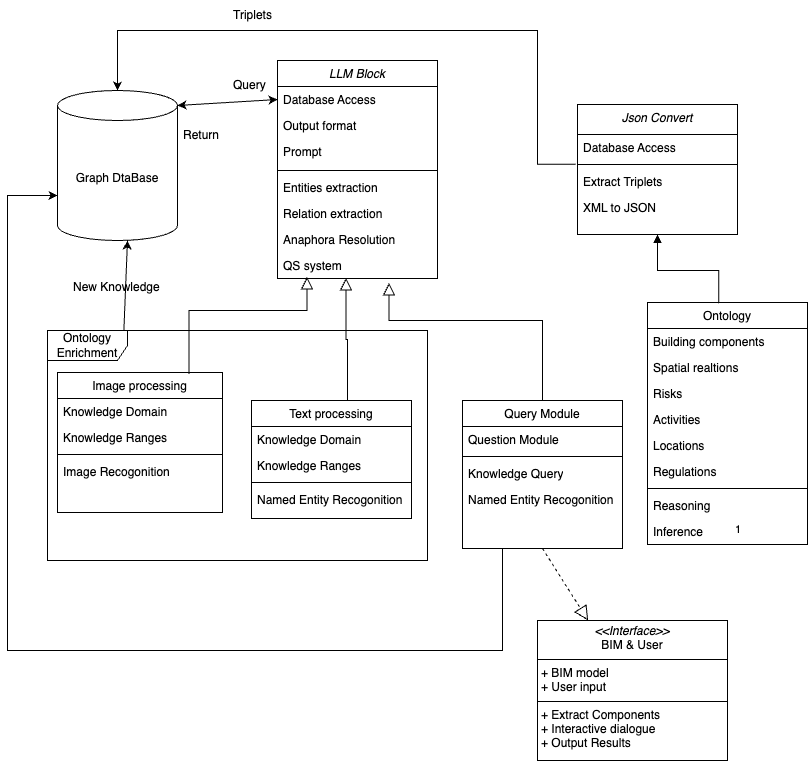
\includegraphics[width=0.5\textwidth]{figures/uml.png}
    \caption{UML diagram of the methodology: 
    The class: ontology and JSON converter are used to construct the initial ontology framework and store it in the graph database. 
    The ontology enrichment frame are used to identify potential object properties and entities from multimodal data sources, and enrich the data properties of the ontology. The class Query Module are responsible for Question and Answering system and report generation.}
    \label{fig:uml_diagram}
\end{figure}


Our system consists of three components: 
\begin{enumerate}
    \item \textbf{Ontology Framework Construction:}
    
    % We do not rely on large language models (LLMs) to construct the ontology from scratch. 
    % Instead, we create a predefined ontology that defines the domain and ranges of building renovation activities, object properties, 
    % and data properties. This ontology is converted into JSON format and stored in graph databases.
    At the beginning, we construct a predefined ontology regulating the domain and range of classes, object properties, and data properties for safety management in renovation activities.
    The predefined ontology is converted to JSON format and stored in a graph database. 
    
    \item \textbf{Data-Driven Ontology Construction:}
    Data-driven methods are employed to enrich the predefined ontology in two ways:
    \begin{enumerate}
        \item We use LLMs to extract potential object properties and entities from multimodal data sources. These are converted into RDF triples and stored directly in the graph database.
        \item Statistical analysis is performed on the extracted data to enrich the data properties of the ontology. The enriched attributes are then stored in the graph database.
    \end{enumerate}
    \item \textbf{Knowledge Inference:}
    A Retrieval-Augmented Generation (RAG) based method is used to perform knowledge inference and 
    generate reports for safety management in renovation activities. 
    Building Information Modeling (BIM) components are mapped to the ontology through anaphora resolution, 
    and the RAG model interacts with the graph database to generate safety management reports.
\end{enumerate}
\subsection*{Ontology Framework Construction}
\label{sec:ontology_coarse}
% list the standford seven steps for ontology construction
% point out the domain and range of ontology classes and properties are reused from existing ontology
% we use llm only to enrich the ontology from step 4, that is to extract potential object properties and entities
% identify ontology instances and properties, we will not involve in the creation of new classes and define the hierarchy of classes, 
% which is very professional and have high risks, since reliability is not gurananteed, and it is possible to introduce bias
\subsubsection{Ontology Construction}
According to the Stanford seven steps for ontology construction \cite[]{noy2001ontology}, 
the ontology construction process consists of seven steps: \textbf{1.} Define the domain and scope of the ontology, 
\textbf{2.} Consider reusing existing ontologies, 
\textbf{3.} Enumerate important terms in the ontology, 
\textbf{4.} Define the classes and the class hierarchy, 
\textbf{5.} Define the properties of classes, 
\textbf{6.} Define the facets of properties, and
\textbf{7.} Create instances of classes and properties.

Based on literatures, we create a predefined ontology that defines the domain and range of ontology classes and properties for safety management in renovation activities.
The initial ontology framework defines the domain and range of ontology classes and properties. Based on the listed entities and types of relations,
LLMs can extract potential object properties and entities from multimodal data sources to enrich the ontology. 
We also reuse the properties and instances of existing ontologies. The knowledge reasoning is performed on Protégé using semantic web rule language (SWRL) and knowledge reasoning engines like Jena or JESS.
The basic ontology structure is show in Figure \ref{fig:ontology_structure}.
\begin{figure}[htbp]
    % define the figure title
    \label{fig:ontology_structure}
    \centering 
    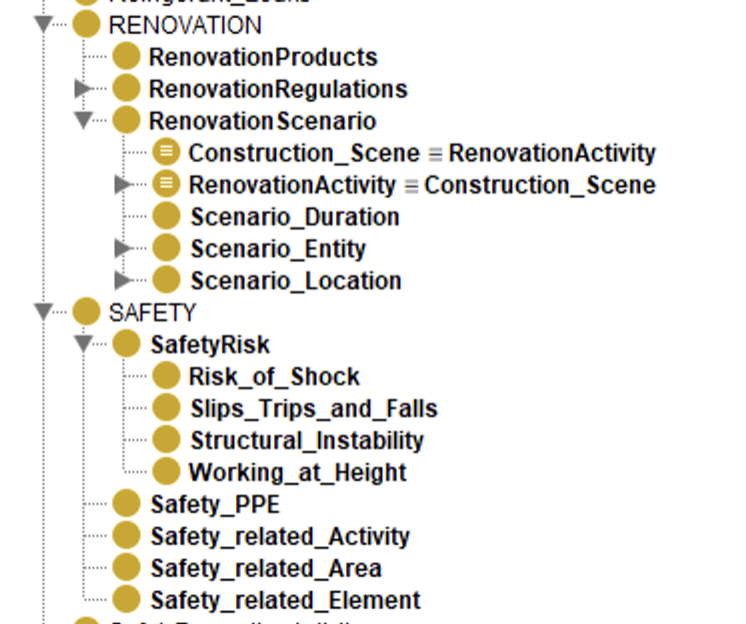
\includegraphics[width=0.5\textwidth]{figures/ontology.png}
    \caption{Ontology structure}
\end{figure}

% define the pseudo code of ontology conversion here
\subsubsection{Ontology format conversion}
Since the owl format mainly used by Protégé only, for the convenience and speed of data storage and retrieval, we convert the ontology to JSON format and store it in the graph database.
The conversion prcess follows the following princples:
\begin{enumerate}
    \item All the relations can be represented as a triplets, in the format \((O,P,S)\), where the \(O\) is the object, \(P\) is the property, and \(S\) is the subject.
    The triplets are stored in graph databases. The object and subject are two nodes, and the property is the edge connecting the two nodes.
    The data properties for each class are stored as attributes of the node in graph databases. The hierarchy of classes is stored as the parent-child relationship in the graph database.
    \item The children of classes should inherit the properties of their parent classes.
    \item There should be no two same nodes in the graph database.
\end{enumerate}
Following the above principles, we convert the ontology to JSON format and store it in the graph database. 

The conversion process can be recursively conducted on the ontology classes and properties. Since the classes and properties in owl is stored hierarchically,
we first extract the direct properties of the class and then add the properties of the parent class to current class. 
We store the properties as a key-value pair in the JSON format.
 Then, we recursively call the function to convert the children of the class until there are no children class left.
The pseudo code of the owl2json is shown in Algorithm \ref{alg:ontology2json}.
\raggedright
\begin{algorithm}
    \begin{algorithmic}[1]
        \label{alg:ontology2json}
        \Require $ontology$
        \Ensure $json\_ontology$
        \State $json\_ontology \leftarrow \{\}$ 
        \Function{ontology2json}{$ontology,json\_ontology$}
            \For{$class$ in $ontology$}
                \State $json\_ontology[class] \leftarrow \{\}$
                \For{$property$ in $class$}
                    \State $json\_ontology[class][property] \leftarrow \{\}$
                    \For{$value$ in $property$}
                        \State $json\_ontology[class][property].append(value)$
                    \EndFor
                \EndFor
            \EndFor
            \Return $json\_ontology$
        \EndFunction
        % \textbf{Function} $ontology2json(ontologyClass, ParentProperties, JsonFile)$
        %     \FOR{$property$ in $ontologyClass.properties$}
        %         \STATE $JsonFile[ontologyClass][property] \leftarrow ontologyClass.property$
        %         \STATE $JsonFile[ontologyClass][property].append(ParentPropertie[property])$
        %         \STATE $JsonFile[ontologyClass][property] \leftarrow ontologyClass.property$
        %         \STATE $JsonFile[ontologyClass][property].parentParentPropertie.parentName$
        %     \ENDFOR 
        %     \FOR{$child$ in $ontologyClass.children$}
        %         \STATE ontology2json($child, JsonFile[ontologyClass][property], JsonFile$)
        %     \ENDFOR
        %     \textbf{return} $JsonFile$   
        % \Procedure{ontology2json}{$ontology$}
        %     \FOR{$class$ in $ontology$}
        %         \STATE $json\_ontology[class] \leftarrow \{\}$
        %         \FOR{$property$ in $class$}
        %             \STATE $json\_ontology[class][property] \leftarrow \{\}$
        %             \FOR{$value$ in $property$}
        %                 \STATE $json\_ontology[class][property].append(value)$
        %             \ENDFOR
        %         \ENDFOR
        %     \ENDFOR
        %     \RETURN $json\_ontology$
        % \EndProcedure


        \For{$class$ in $ontology$}
            \State $json\_ontology[class] \leftarrow \{\}$
            \For{$property$ in $class$}
                \State $json\_ontology[class][property].append(property) \leftarrow \{\}$   
            \EndFor
            %\State ontology2json($class, json\_ontology[class][property], json\_ontology$)
            % call the function here
            \State $json\_ontology \leftarrow \Call{ontology2json}{class,json\_ontology}$
        \EndFor
        % add comment here in pseudo code


    \end{algorithmic}
\end{algorithm}
After we convert the ontology to JSON format, we store it in the graph database directly using the graph database API and merge the repeatitive nodes in the graph database.
Compare the XML format of the Graph database storation and JSON format of ontology,
 the JSON format is more readable and easy to store and retrieve. 
 Comparing the time to retrieve properties of a class, the JSON format is also faster than XML format in python.
 The detailed comparison is shown in Table % \ref{tab:format_comparison}.


\subsection*{Data-Driven Ontology Construction}
\label{sec:ontology_fining}
In this step we will apply the LLMs to enrich existing ontology. 
Due to the limitation of data, we only design LLM to enrich ontology in two aspects, \ref{tab:ontology_enrichment} :
\begin{table}[htbp]
    \centering
    \label{tab:ontology_enrichment}
    \caption{LLM based ontology enrichment}
    % make table alignment with text
    
    \begin{tabular}{ccc}
        \hline
        \textbf{Domain} & \textbf{Type of Properties} & \textbf{Input format} \\
        \hline
        Risk Frequency  &  Data Property              &  image               \\
        Related Regulation & Object Property           &  text document        \\
        \hline

    \end{tabular}
\end{table}
\subsubsection{Risk Frequency}
The risk frequency is a data property that describes the frequency of risks in renovation activities. 
Current ontology only defines the potential risks related to renovation activities, 
but all kinds of risks share the same weight in the ontology.
We use LLMs to extract the risk frequency from related image from related image database.
The enrichment proces follows the following steps:
\begin{enumerate}
    \item \textbf{Define the range of risks: } \\
    As all possible risks are defined related to renovation activities are all defined in the ontology, 
    we make the LLMs to conduct semantic analysis on the images related to targeted activites. 
    \item \textbf{LLM prompt Tuning: } \\
    We select few images for prompt tuning to make the response of the LLMs more accurate and reliable. 
    The process of prompt tuning is as shown in 


    For stable experiment results, we set the temperature of the LLMs to be 0.1,
     since the higher temperature may introduce randomness to the results, which will affect the reliability of the results.
    \item \textbf{Extract the risk frequency: } \\
    We count the identified risks' frequency in the images and store the frequency as the data property of the ontology.
    If the risk is not related to the renovation activities, we will add the relation to the ontology and write to the graph database.
\end{enumerate}

We display the workflow of the risk frequency extraction in Figure \ref{fig:risk_frequency_workflow}. and samples of risk frequency enrichment in Table \ref{tab:risk_frequency_sample}.
After we store the data in graph database, we can query the frequency of all identified risks related to the renovation activities, see figure \ref{fig:risk_frequency_query}.
\begin{figure}
    \label{fig:risk_frequency_query}
    \centering
    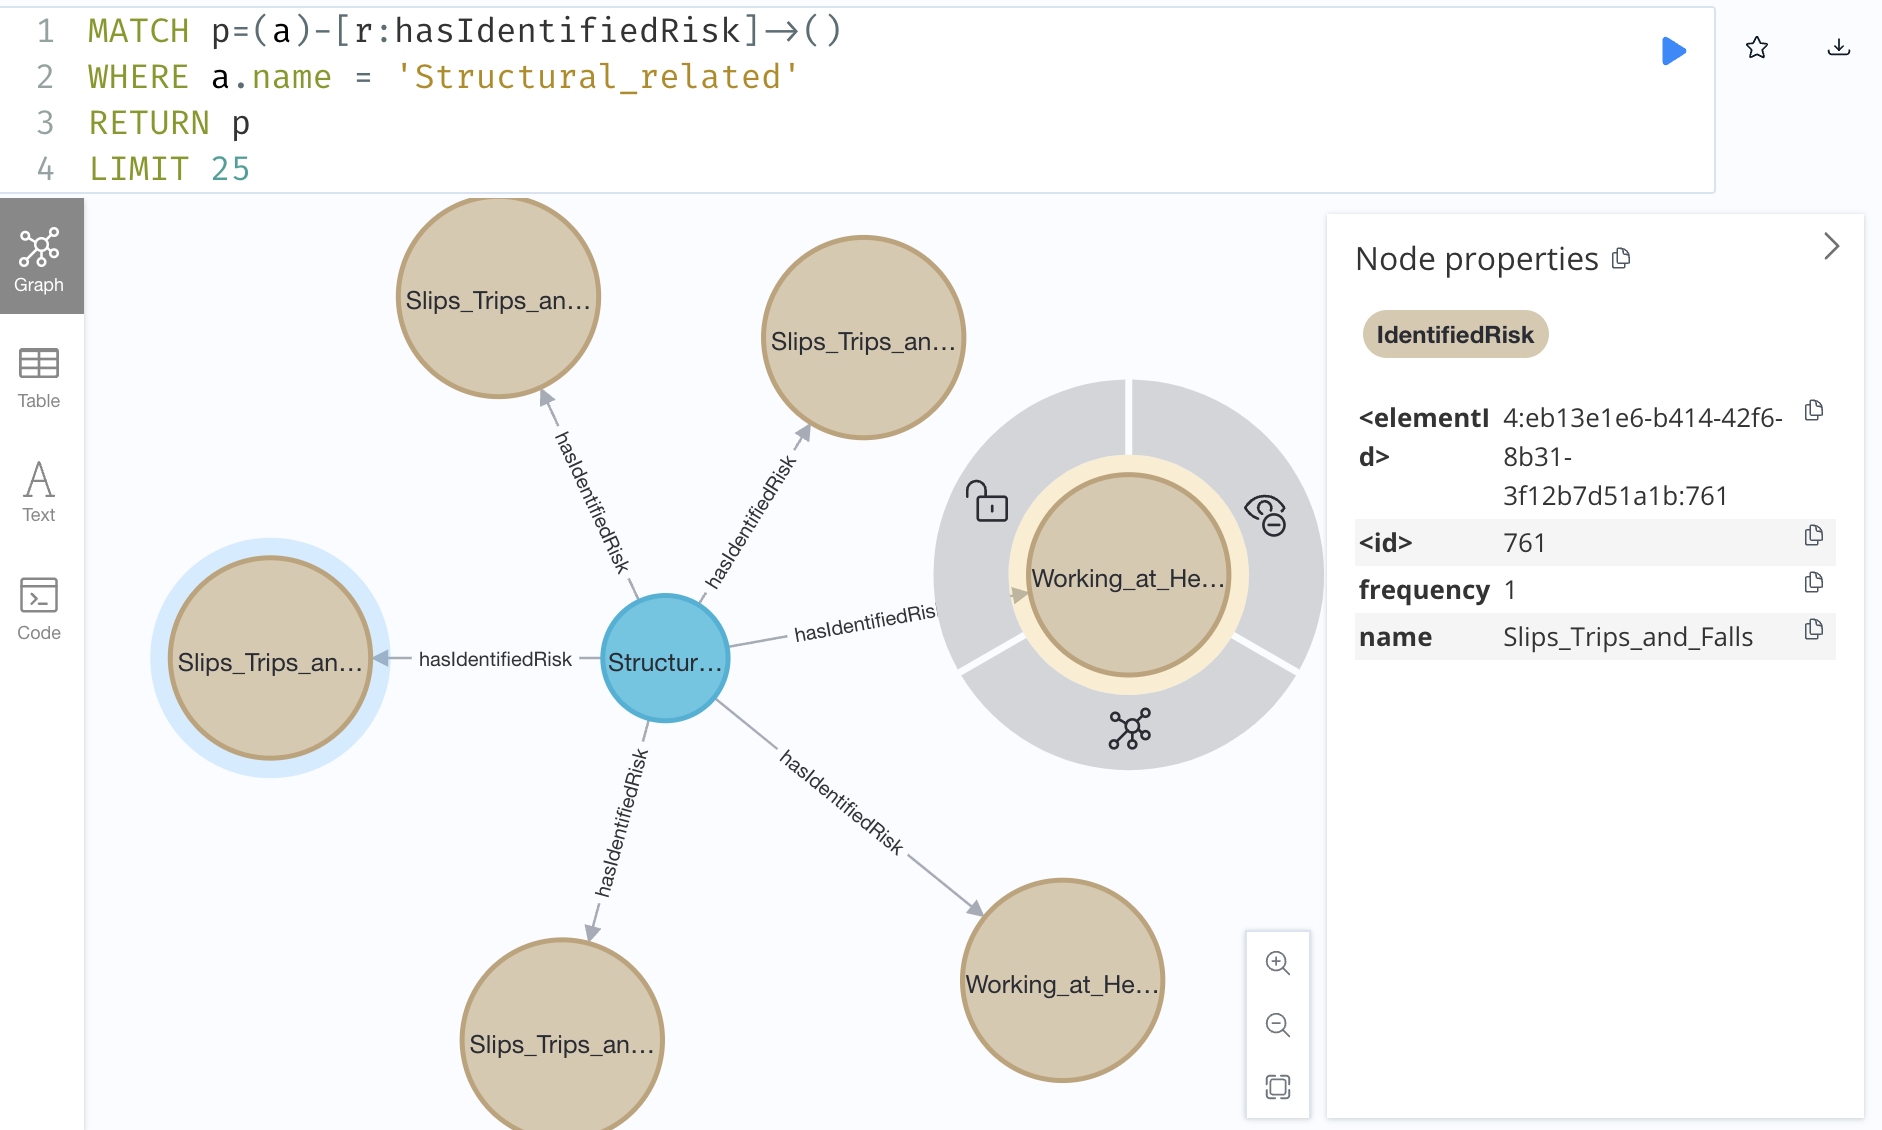
\includegraphics[width=0.5\textwidth]{figures/graph_frequency_query.png}
    \caption{Risk frequency query in graph database: The risk frequency attribute on the risk node indicate the class of risk frequency in related renovation activities.
     The higher number indicates the higher frequency of the risk in the renovation activities.}
\end{figure}

\begin{figure}
    \label{fig:risk_frequency_workflow}
    \centering
    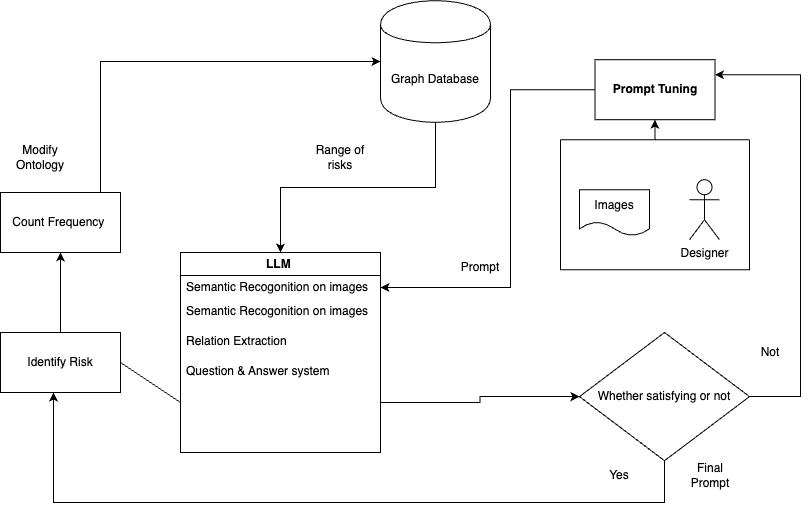
\includegraphics[width=0.5\textwidth]{figures/Data properties enrichment.png.png}
    \caption{Risk frequency extraction Workflow}
\end{figure}
% Here is a sample for activity risk frequency extraction:
\begin{table*}[htbp]
    \centering
    \label{tab:risk_frequency_sample}
    
    \begin{tabularx}{\textwidth}{ccX}
        \hline
        \multicolumn{3}{c}{Prompt setting} \\
        \hline
        %left align the text
        \multicolumn{3}{l}{Identify risks appear in the following image. The scope of risks are: \textless risks range \textgreater } \\
        \multicolumn{3}{l}{only return the name of the risks that are present in the images,} \\
        \multicolumn{3}{l}{the format should be JSON. The outputs should be organized in} \\
        \multicolumn{3}{l}{the format of risks:[risk1,risk2,risk3]} \\
        \hline
        \textbf{Activity} & \textbf{Image} & \textbf{Identified Risks} \\
        \hline
        Ductwork\_removal & 
        \raisebox{-\totalheight}{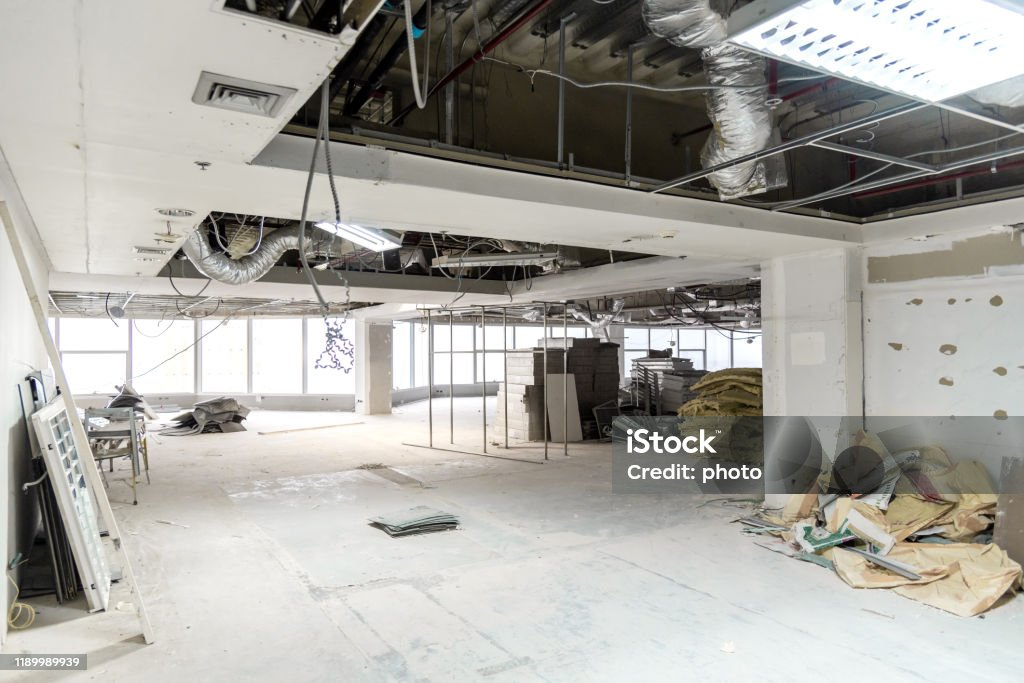
\includegraphics[width=0.3\textwidth]{figures/remove-hvac.jpeg}} 
        & Working\_at\_Height, Falling\_Objects,Slips\_Trips\_and\_Falls, Dust\_and\_Debris \\
        \hline
        Structural\_related & 
       \raisebox{-\totalheight}{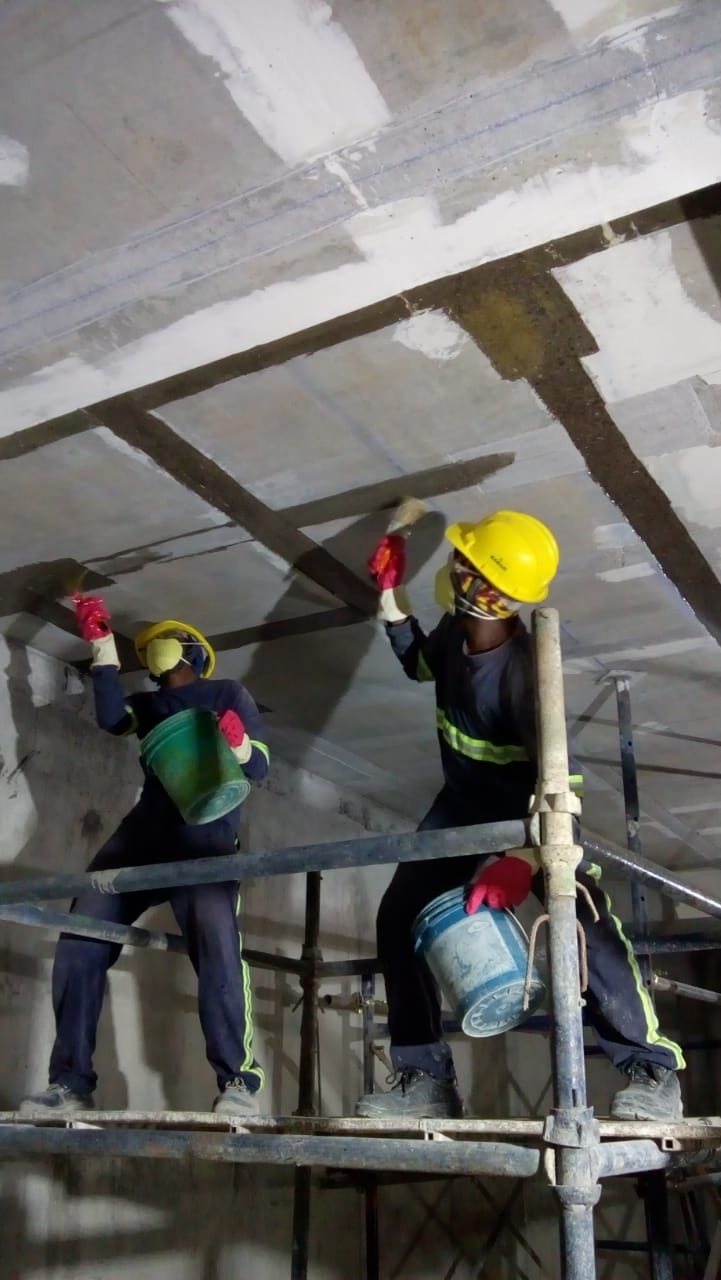
\includegraphics[width=0.3\textwidth]{figures/p.jpeg}} 
        & Working\_at\_Height, Slips\_Trips\_and\_Falls \\
        % 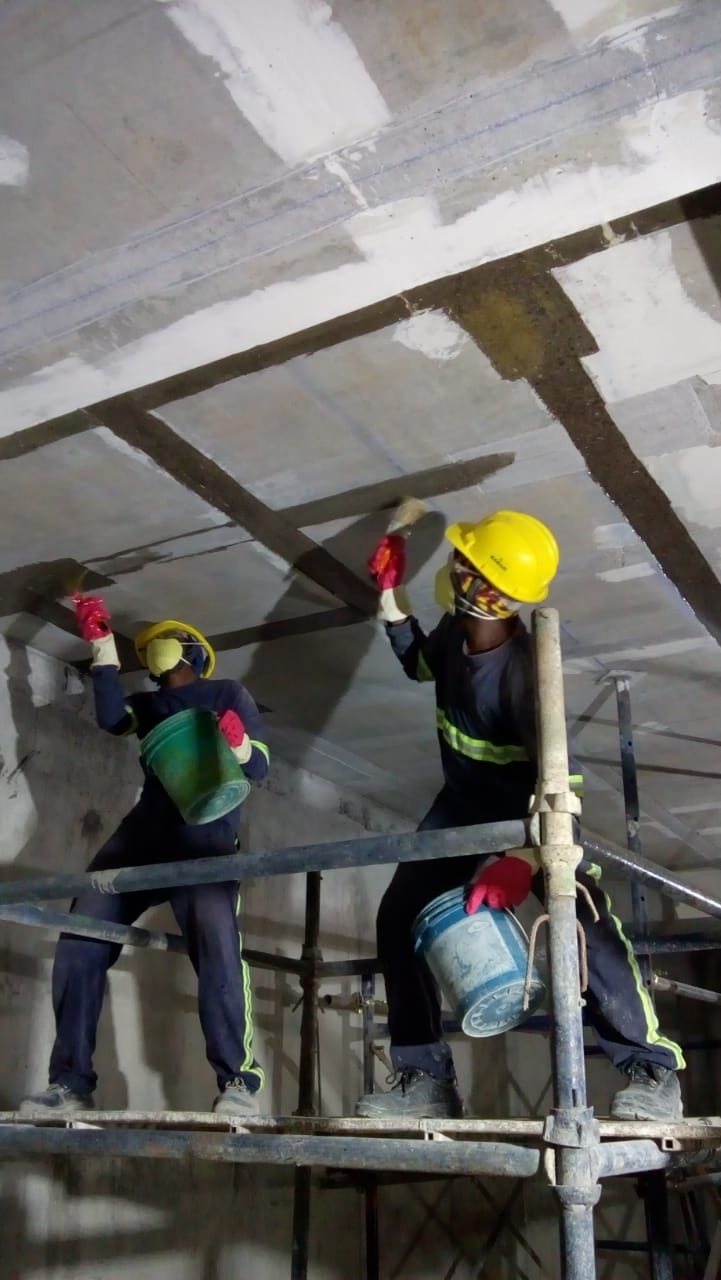
\includegraphics[width=0.1\textwidth]{figures/p.jpeg}
        %  & Working_at_Height, Slips_Trips_and_Falls \\
        \hline
        Site\_Clearing & 
        
        \raisebox{-\totalheight}{\includegraphics[width=0.3\textwidth]{figures/2024-05-31-5.41.36.png}}
         & Falling\_Objects, Slips\_Trips\_and\_Falls, Dust\_and\_Debris \\
        \hline
    \end{tabularx}
    \caption{Risk frequency enrichment sample}
\end{table*}
\subsubsection*{Regulation Document Processing} 
Applying NLP for information extraction has two branches: traditional methods and deep learning-based methods.
In safe management in building construction area, 
except few study applying machine-learning based methods for information extraction \cite[]{marucci2017classifying},
most of the studies are applying traditional NLP methods for information extraction \cite[]{xu2021extracting,wu2024nlp}. 
Reviewing previous studies, the machine-learning based methods need to train a text classifier based on SVM or naive bayes \cite[]{marucci2017classifying};
the traditional NLP need to setting linguistic rules to extract key word from sentences and have requirement for the quality of the text \cite[]{xu2021extracting,wu2024nlp}.

In our study, we apply Large language model to achieve information extraction from text documents, compared with previous studies,
large language model has two advantages: \textbf{1. High generalization:} 
the large language model can extract information from text documents without setting linguistic rules, only setting the prompt for the model;
\textbf{2. High flexibility:} the large language model can extract information from text documents with different quality, since the model is trained on large corpus of text data.

The process of information extraction is as follow:
\begin{enumerate}
    \item \textbf{Define the range of activities and entities: } \\
    From the graph database we extract the range of all possible activities and entities related to the input regulation documents. 
    \item \textbf{Identify the activities relted to the regulation: } \\
    Identify all possible activities related to the regulation documents
    \item \textbf{Identify the entities related to the activities: } \\
    Given each identified activity, we hope that we can also identify the entities involved in the activities, such as 
    building slabs, ceillings, cranes and so on.
    \item \textbf{LLM prompt Tuning: } \\
    Given the sample of regulation documents we continue to tune the LLM prompt to make the response of the LLMs more accurate and reliable.
    \item \textbf{Extract the related regulation: } \\
    We extract the related activities and entities involve in the activity from regulation document and store the information in the graph database.
\end{enumerate}

The process of related regulation extraction is shown in Figure \ref{fig:related_regulation_workflow}.
\begin{figure}
    \label{fig:related_regulation_workflow}
    \centering
    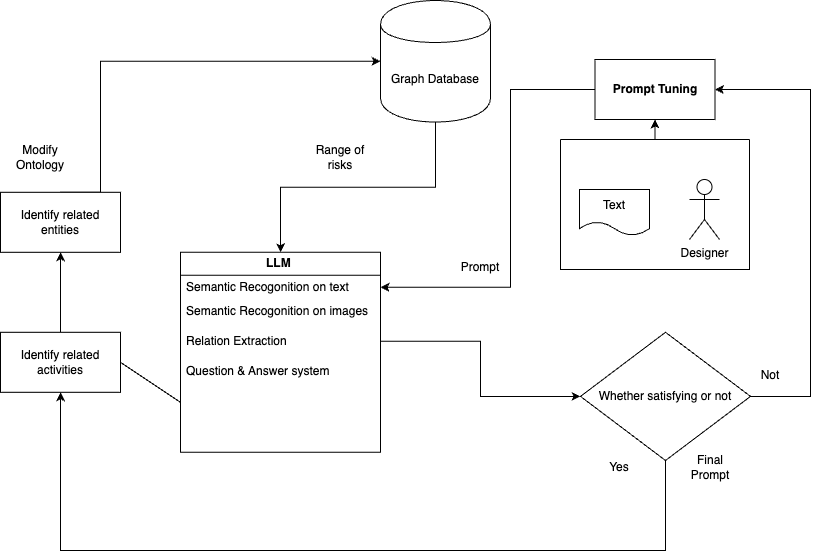
\includegraphics[width=0.5\textwidth]{figures/text_extraction.png}
    \caption{Regulation Document processing Workflow}
\end{figure}

The regulation document processing results is shown in Table \ref{tab:related_regulation_sample}. %add a footnote that the regulation1,2,3 are in the appendix
And the final output on the graph database is shown in Figure \ref{fig:related_regulation_query}.
\footnote{the document of regulation1,2,3 are in the appendix}

\begin{table*}
    \centering
    \label{tab:related_regulation_sample}
    \begin{tabularx}{\textwidth}{cX}
        \hline 
        \multicolumn{2}{c}{Prompt setting} \\
        \hline
        \textbf{Regulation Document} & \textbf{Identified Activity:[entities]}  \\
        \hline
        regulation1 & Floor\_Slab\_removal:[Concrete\_Foundation\_Slab],Reinforcing\_Bars\_removal: [Reinforcing\_Bars]  \\
        \hline
        regulation2 & Demolition\_Activity:[ Mechanical\_Equipment,Floor,Working\_Surfaces,Cranes,Derricks]  \\
        \hline
        regulation3 &  Structural\_demolition:[Nominal\_Breaking\_Strength, Crane\_Boom, Loadline,SwivelType\_Connection, Steel\_Members, Roof\_Cornice] \\
    \end{tabularx}
    % add a footnote that the regulation1,2,3 are in the appendix
    \caption{Related Regulation extraction sample}
\end{table*}

\begin{figure}
    \label{fig:related_regulation_query}
    \centering
    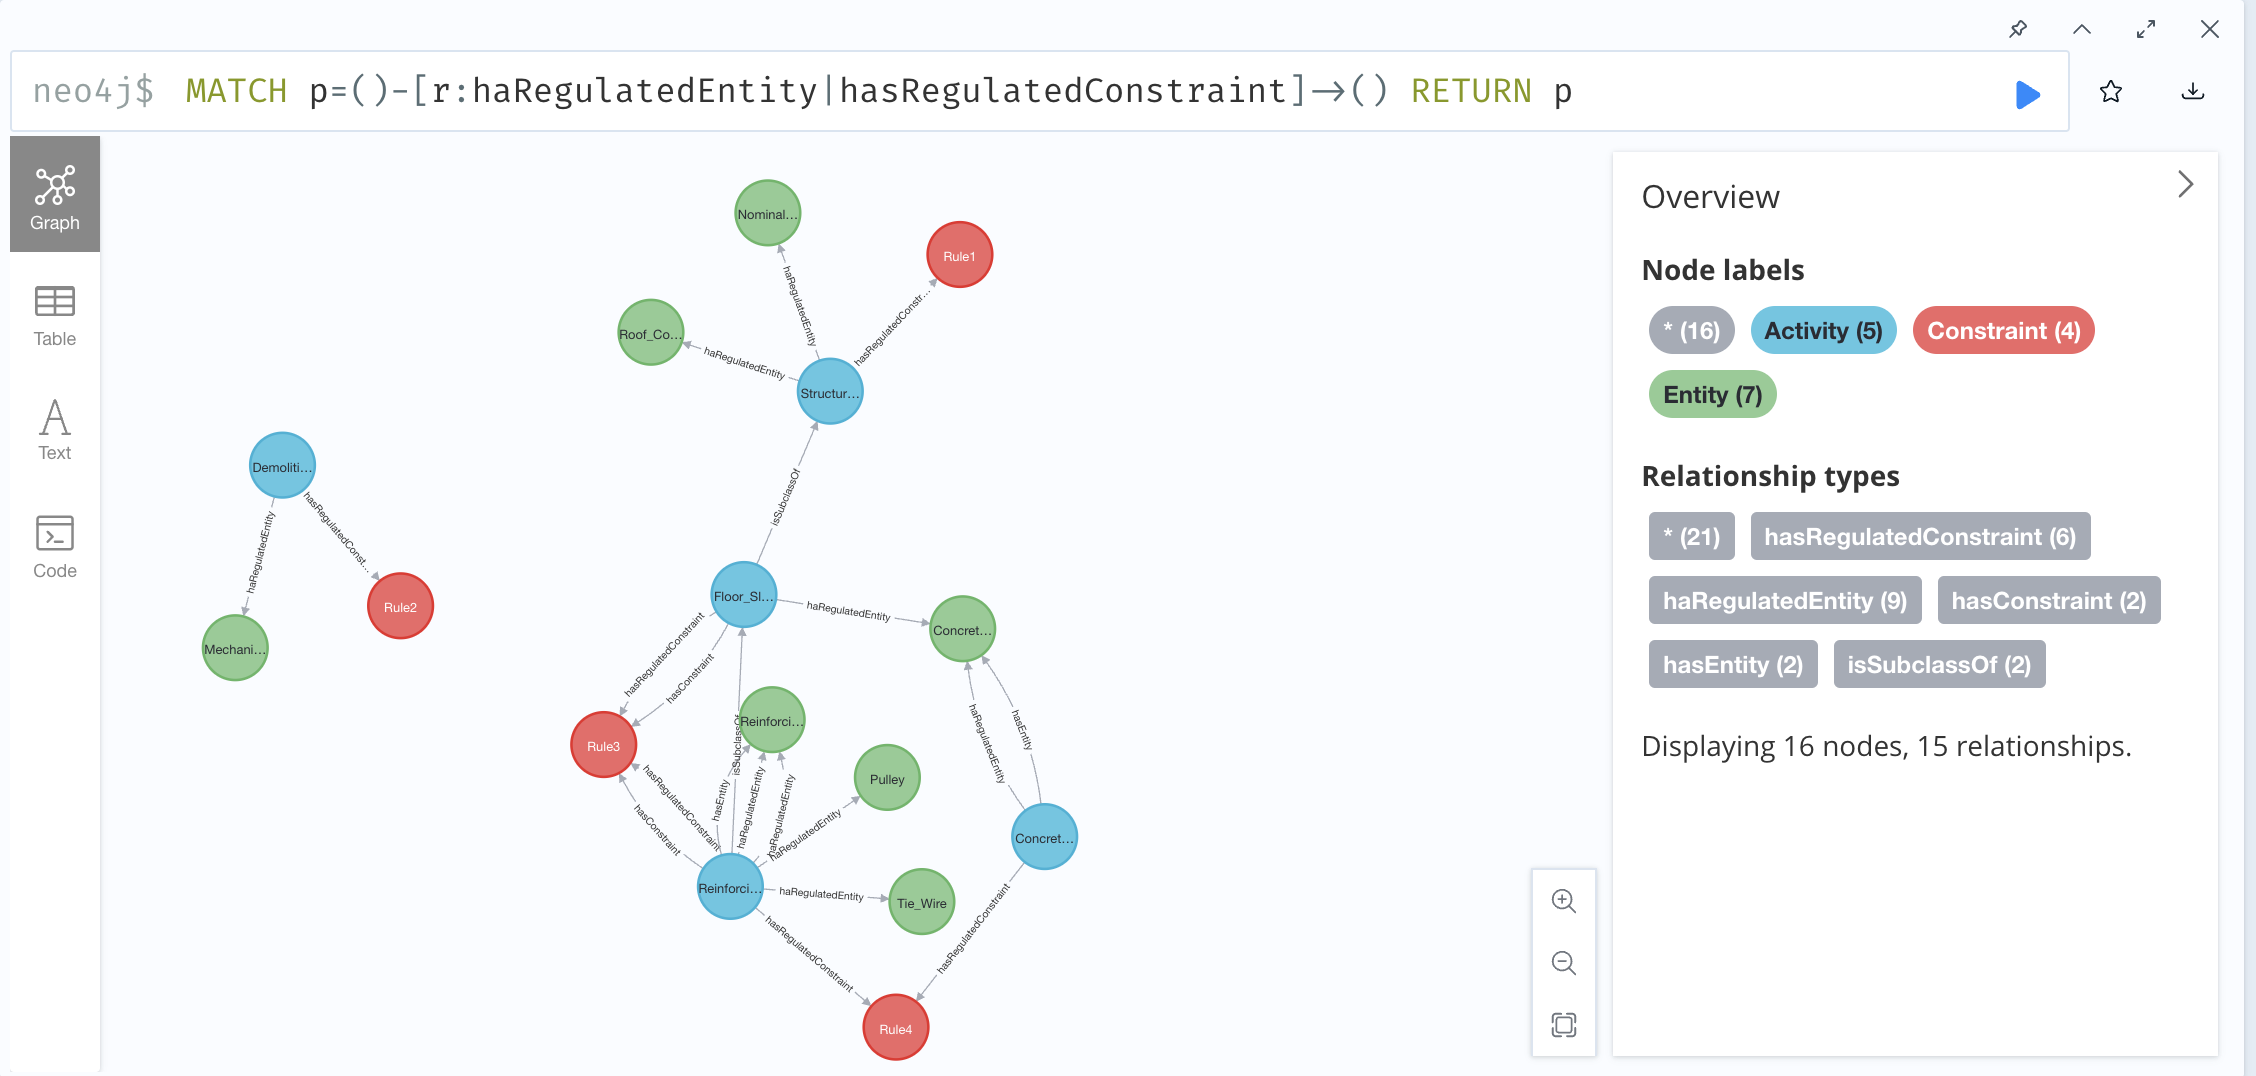
\includegraphics[width=0.5\textwidth]{figures/regulation relation.png}
    \caption{Related Regulation query in graph database: The related activities and entities are stored in the graph database.}
\end{figure}

\subsection*{Knowledge Inference}
\label{sec:knowledge_inference}
% define the RAG model
The final step is to build a Question and Answering system and report generation system based on the ontology.
The input will be the question and answer between user and system, and the BIM model of the renovation activities.
The output will be the report of the safety management in renovation activities. 
The report will contains the following information:
\begin{itemize}
   \item \textbf{Activity: } 
   Based on the components of the BIM model and question and answer between user and system,
    the system will identify the activities related to the renovation activities.
    And the system will also list the entities involved in the activities such as building slabs, ceillings, cranes and so on.
    \item \textbf{Risk: }
    Based on the identified activities and entities, the system will identify all the potential risks related to the renovation activities.
    Based on the statistical analysis of the risk frequency, the system will also return the statistical analysis of the risk frequency.
    \item \textbf{Regulation: }
    Based on the activities involved in the building renovation, the system will also return the related regulations
    and also the regualted entities included in the regulated activities. 
\end{itemize}

The whole process of Question and Answering system is decomposed into the following steps:
\begin{enumerate}
    \item \textbf{Mapping BIM components to ontology: } 
    Firstly, we extract all the components of the BIM model, and searching the corresponding entities related to the components,
    which are stored in the graph database.
    \item \textbf{Identify the activities: }
    The range of all possible activities are identified based on recogoized entities from the graph database. 
    Firstly, We use the relation $hasEntity$ to match all possible activities from graph database, including demolition and installation activities. 
    Then, we narrow the range of activities based on the question and answer between user and system. 
    Lastly, we display all the identified activities and entities involved in the renovation, 
    if user agree with the identified activities and entities involving in, we continue to the next step,
    otherwise, we will ask user to make supplement to the identified activities and entities, and repeat the process.
    \item \textbf{Identify the risks and regulation: }
    We return information in three aspects:
    \begin{enumerate}
        \item \textbf{Risk: } 
        We return the risk and the frequency of risk related to the renovation activities.
        \item \textbf{Regualtion: }
        We return the related regulations and entities involved in the regulation.
        \item \textbf{Cases: }
        We return the cases related to the high frequency risks and the related regulations.
    \end{enumerate}

    We make LLM summarize the identified risks and regulations and cases, and generate the report for the safety management in renovation activities.
\end{enumerate}

Compared with traditional ontology-based method that use SPARQL query to obtain knowledge from ontology,
We make LLM to interact with user and system and establish mapping between BIM components and ontology. 
The advantages is that: \textbf{1. Objective: } the LLM can process the querying process objectively and accurately,
excluding the bias introduced by human; \textbf{2. High flexibility: } 
The information is passed to the LLM in the form of prompt, which is more flexible and generalizable than the SPARQL query.
User, especially the non-professional user, can easily interact with the system and obtain the information they need.
The workflow of the knowledge inference is shown in Figure \ref{fig:knowledge_inference_workflow}.
\begin{figure}
    \label{fig:knowledge_inference_workflow}
    \centering
    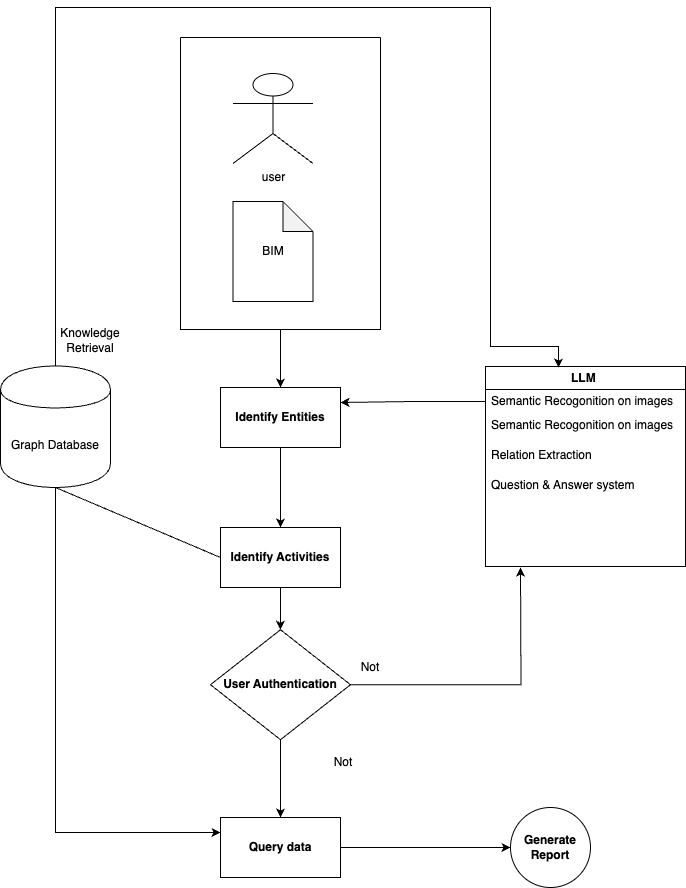
\includegraphics[width=0.5\textwidth]{figures/qa system.png}
    \caption{Knowledge Inference Workflow}
\end{figure}
\subsection{Summary}
In this section, we propose a methodology for safety management in renovation activities based on ontology and multimodal data sources.
We first construct a predefined ontology that defines the domain and range of ontology classes and properties for safety management in renovation activities.
Then, we apply LLMs to enrich the ontology by extracting potential object properties and entities from multimodal data sources.
We also apply LLMs to extract risk frequency from images and related regulations from text documents.
Finally, we build a Question and Answering system and report generation system based on the ontology to support safety management in renovation activities.
The system can interact with users and BIM models to identify activities, risks, and regulations related to renovation activities.
The system can also generate reports for safety management in renovation activities based on the identified information.
The whole workflow is shown in Figure \ref{fig:methodology_workflow}.
\begin{figure*}[htbp]
    
    \label{fig:methodology_workflow}
    \centering
    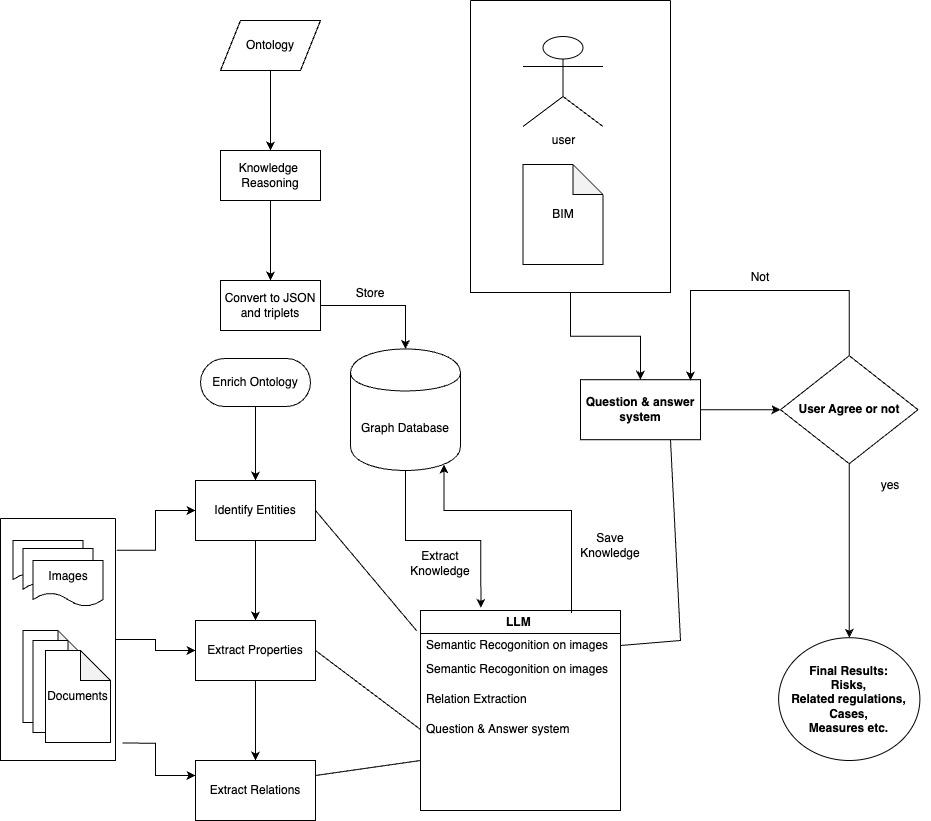
\includegraphics[width=\textwidth]{figures/total workflow.png}
    \caption{Methodology Workflow}

\end{figure*}
\section{Results \& Verification}
\label{sec:results}
% read revit file and 

\subsection*{Input Data and Experiment setting}
The Input Data will be BIM model in Revit format, which is a hospital. We assume that the renovation activity is to install 
a new air conditioning system in the hospital. Here is the BIM model of the hospital (Figure \ref{fig:hospital}).
\begin{figure}
    \centering
    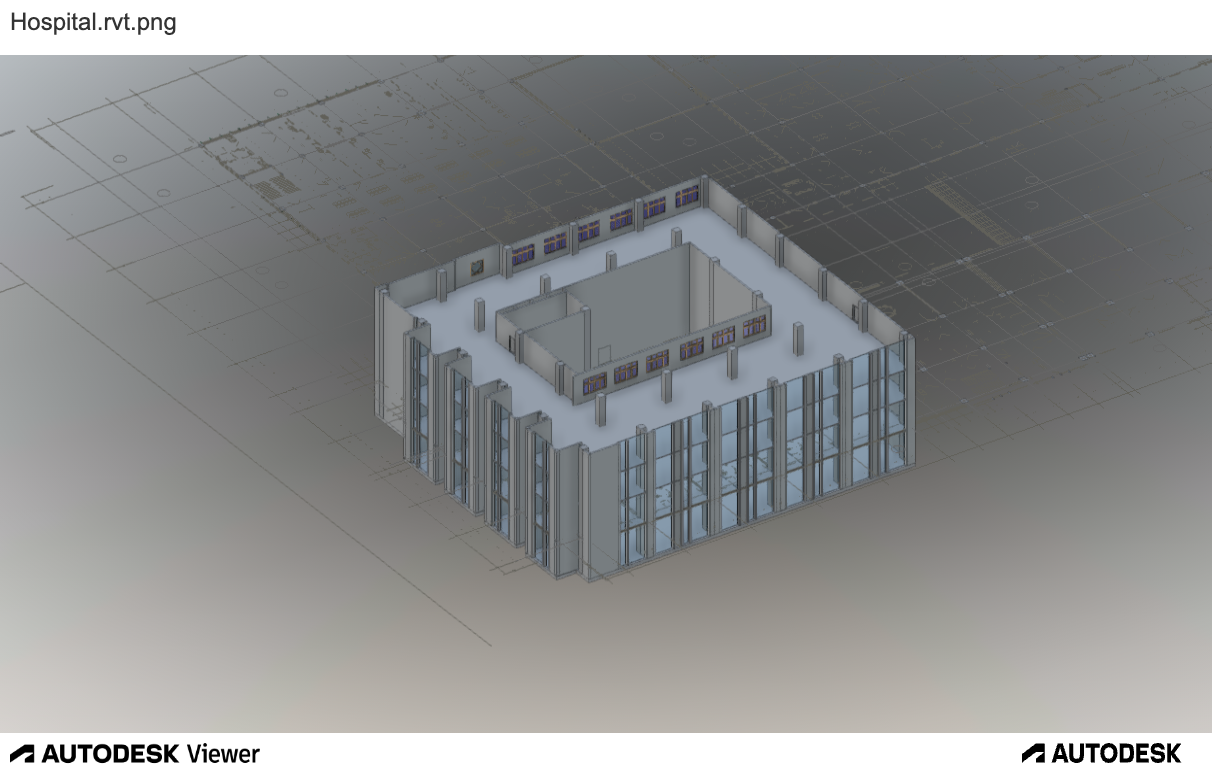
\includegraphics[width=0.5\textwidth]{figures/Hospital.rvt.png}
    \caption{Hospital BIM model}
    \label{fig:hospital}
\end{figure}

The LLM model we choose is OpenAI's GPT-4o. We call the API of GPT-4o in Python environment to build our safety management system.
The platform of Graph Database we choose is Neo4j. We use the Neo4j Desktop to build the graph database and query the graph database.

\subsection{Graph Database Construction}
The first step is converting the ontology to the graph database. The detailed steps is shown in section \ref{sec:ontology_coarse}
Here we should the overview graph of ontology stored in Neo4j (Figure \ref{fig:ontology_graph}).
\begin{figure}
    \centering
    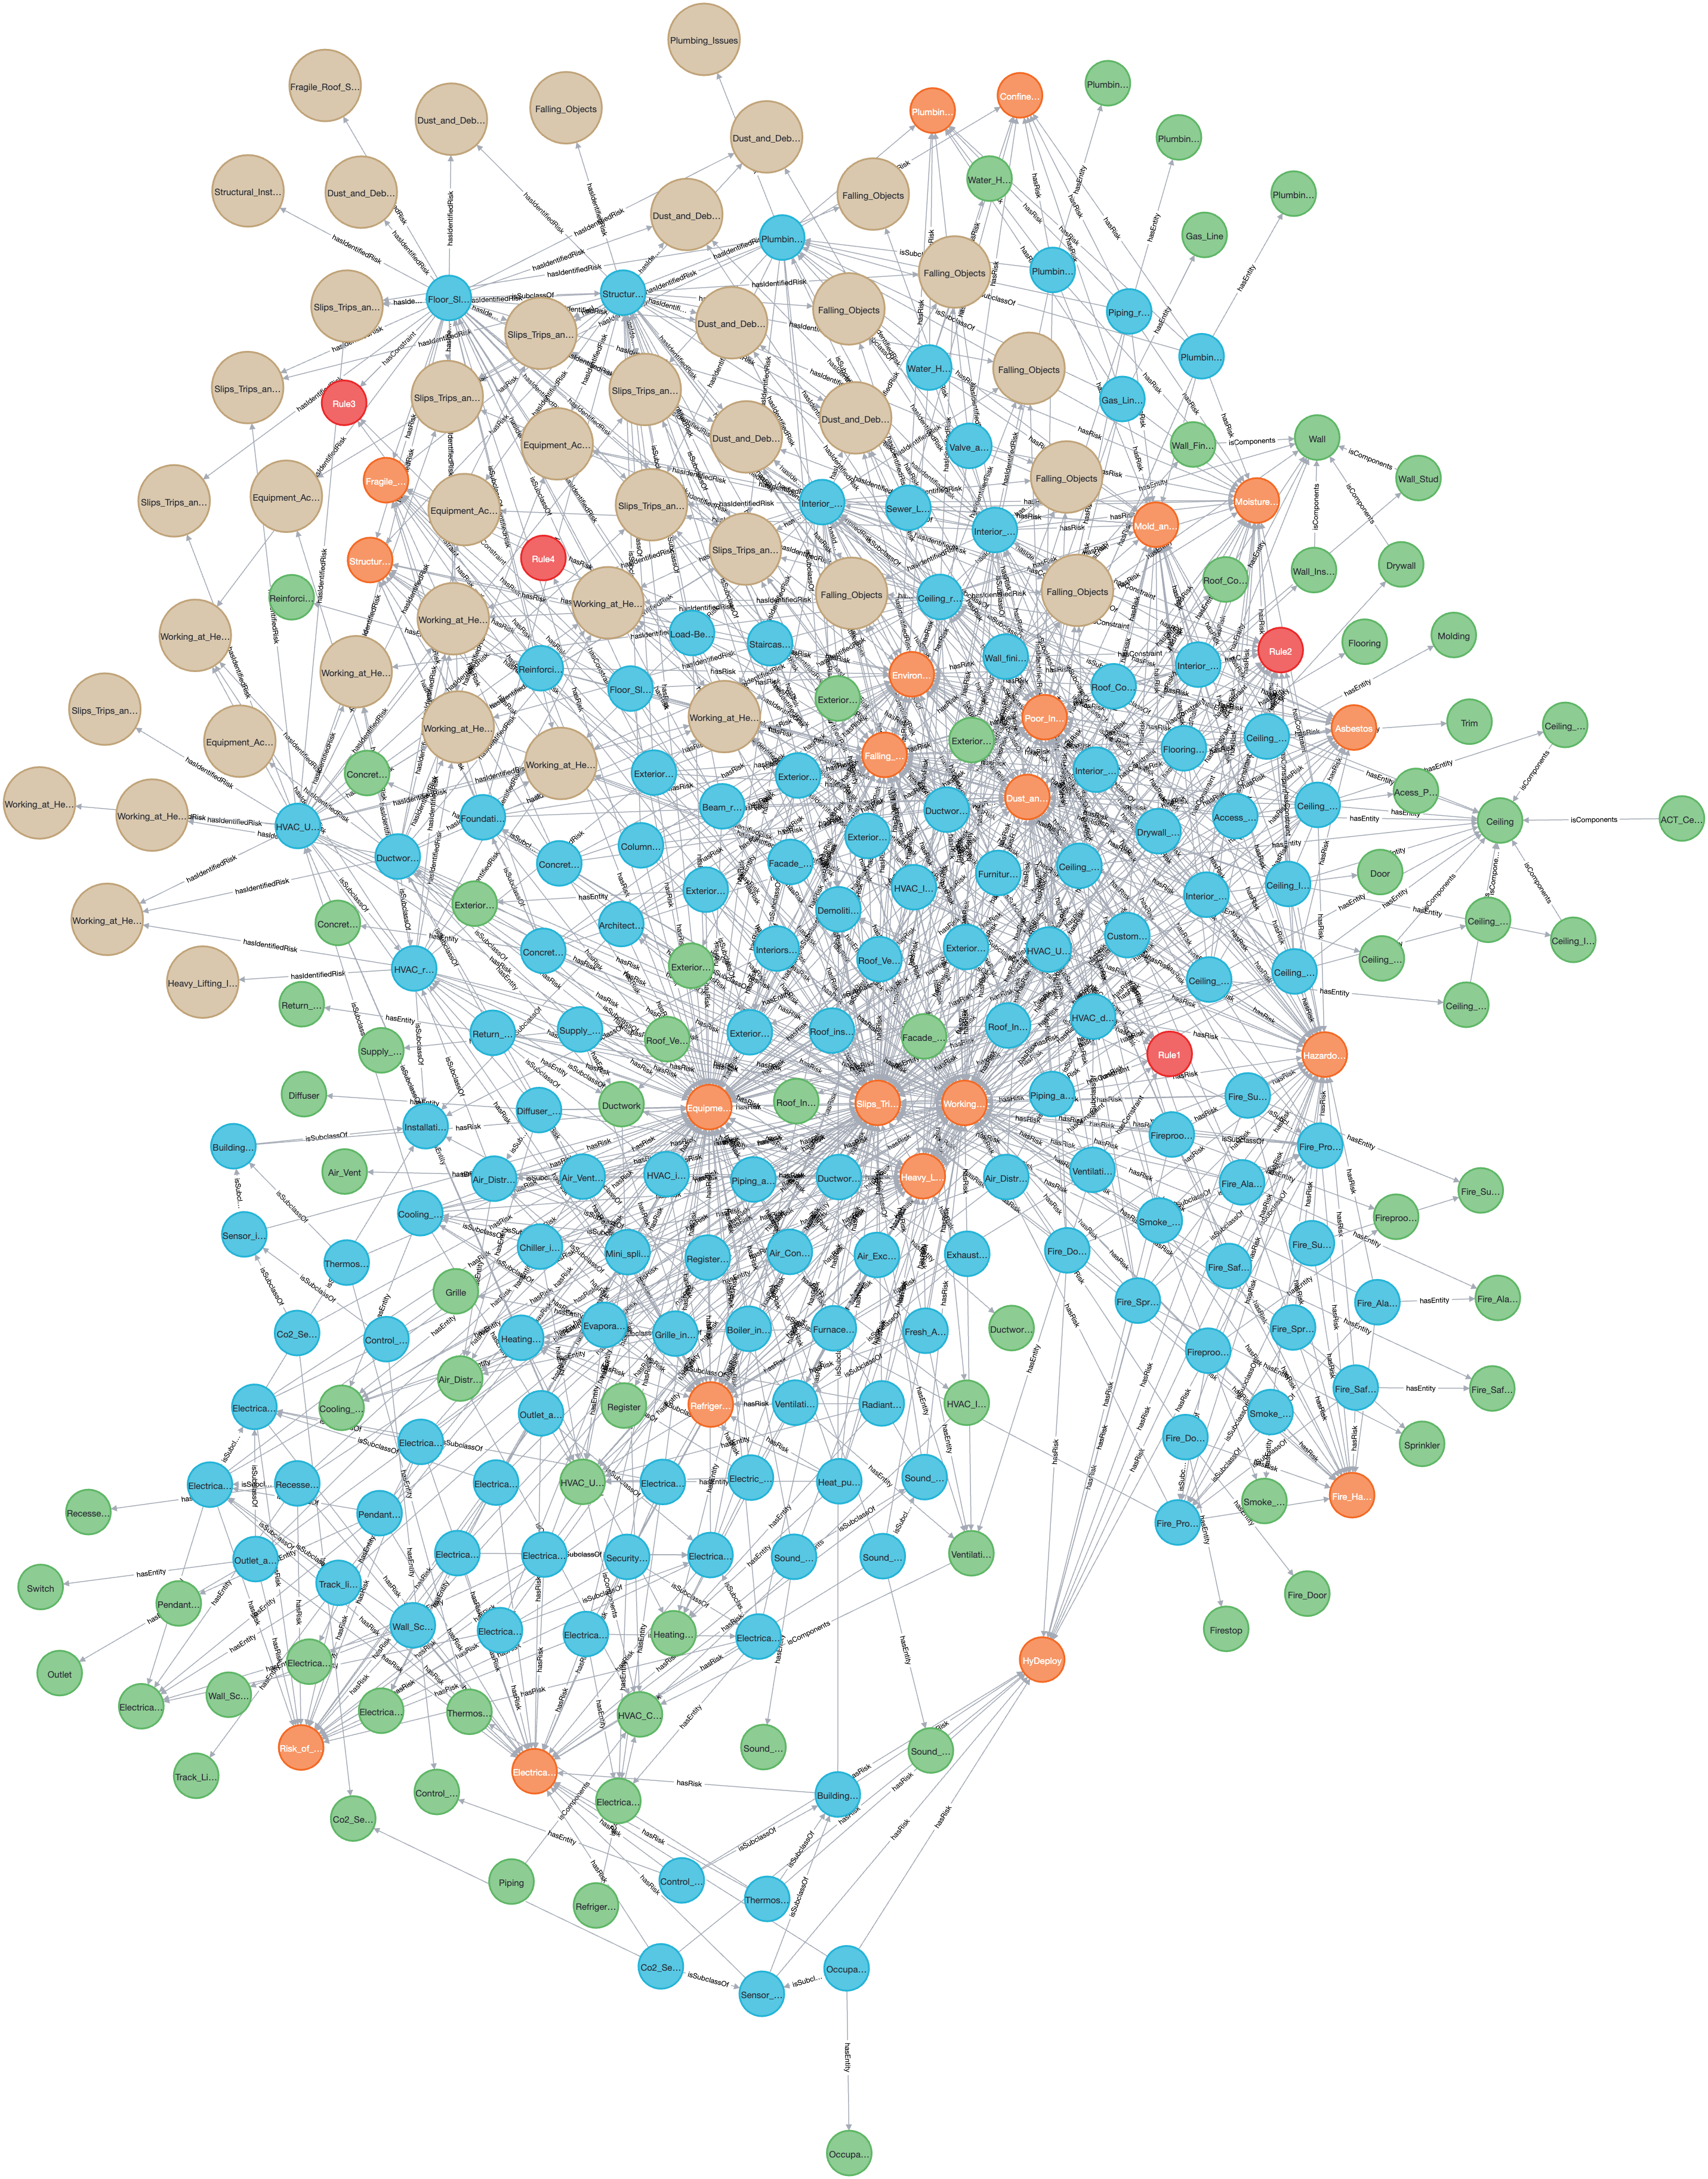
\includegraphics[width=0.5\textwidth]{figures/graph (2).png}
    \caption{Ontology Graph in Neo4j}
    \label{fig:ontology_graph}
\end{figure}
\subsection*{Ontology Enrichment}
We input the images and regulation documents to the LLM model. The LLM model will generate two more relations on original ontology. \\
The first relation is the relation between the renovation activities and the risks.
 There is a new relation called 'hasIdentifiedRisk' between renovation activities and identified risk from collected images on each activited during the renovation process. 
 The same risk may appeared more than once among different images, we will calculate the frequency of each risk appeared in the images. The frequency of each identifed risk will be stored in the attribute of the risk node in graph. 
 
 The second relation is the regulation related to renovation activities. The LLM model will generate a new relation called 'hasRelatedRegulation' between renovation activities and the regulation documents.
 This relation indicates that the regulation is applicable to the renovation activities. Another relation LLM extracted from regulation document is 
 the relation "hasRegulatedEntity", which is relation between activities and entities appeared in the regulation document,
 which indicates that the entities in renovation activities has to be regulated by the regulation document.

\begin{figure}
    \centering
    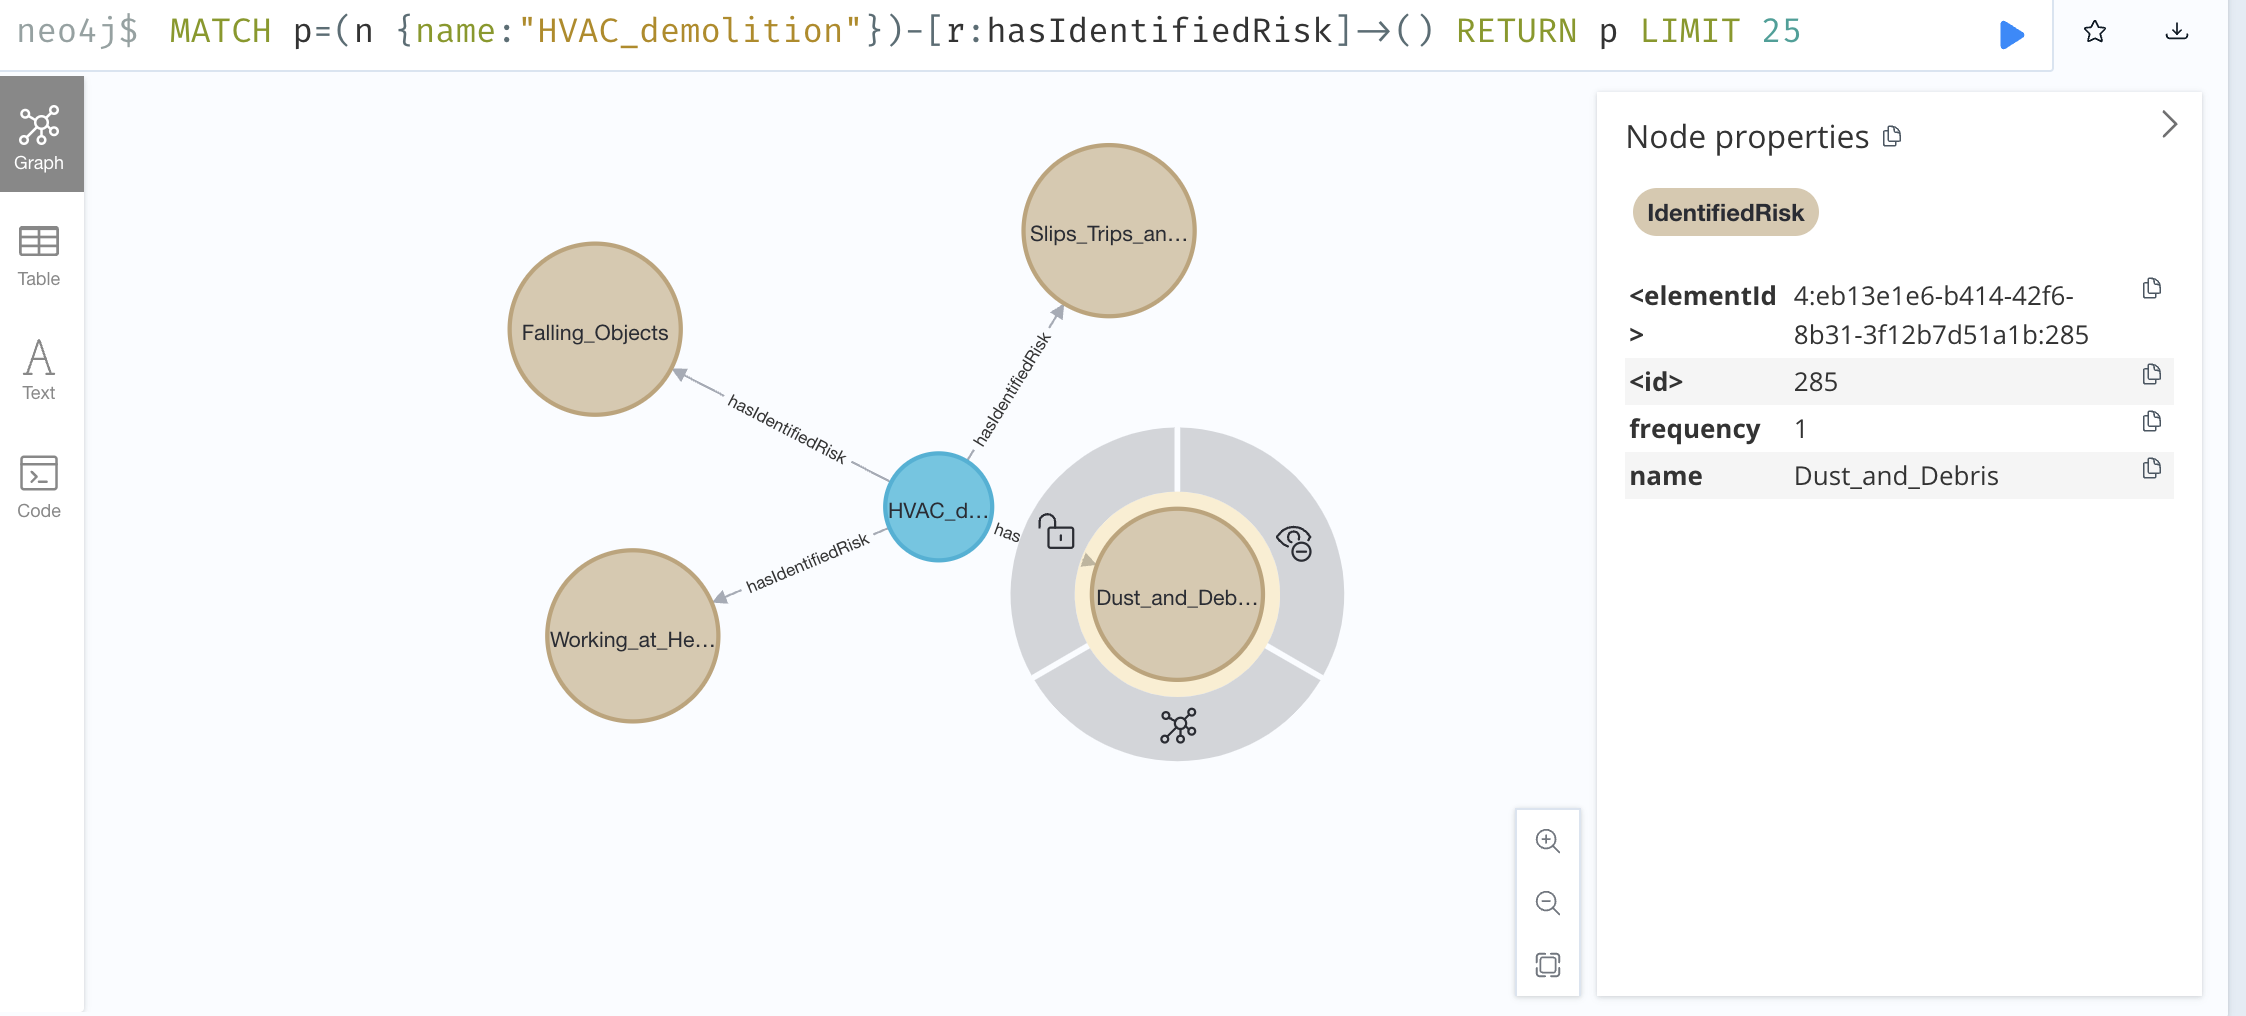
\includegraphics[width=0.5\textwidth]{figures/risk identified.png}
    \caption{Samples of extracted relation from images in Neo4j}
    \label{fig:image_enrichment}
\end{figure}
\begin{figure}
    \centering
    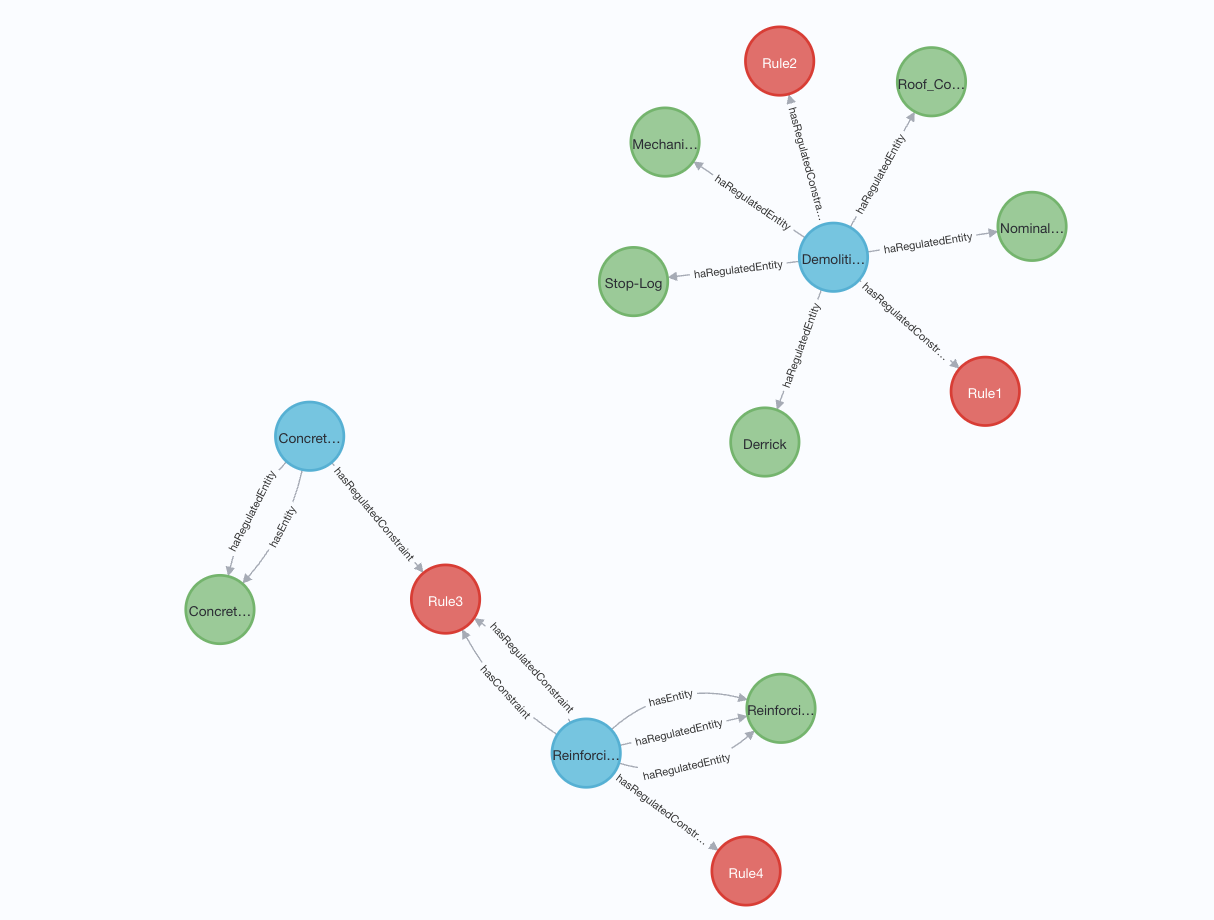
\includegraphics[width=0.5\textwidth]{figures/regulation.png}
    \caption{Samples of extracted relation from regulation documents Neo4j}
    \label{fig:ontology_graph_enriched}
\end{figure}

After the ontology enrichment, the ontology graph in Neo4j is shown in Figure \ref{fig:ontology_graph_enriched,fig:image_enrichment}.
The extracted information can be easily queried from the graph database, given the name of renovation activities involved in the renovation process.

\subsection{The Final Interactive Interface}
The final interactive interface is a QA system, which is run on command line mode. It could be transfer to a web-based platform
or Autodest Revit. But for the convenience of the experiment, we only implement the command line mode.

% the result of the system is still undefine,
The dialogue between the user and the system is shown in the Figure %\ref{fig:dialogue}.
% \begin{figure}
%     \centering
%     \includegraphics[width=0.5\textwidth]{figures/dialogue.png}
%     \caption{Dialogue between the user and the system}
%     \label{fig:dialogue}
% \end{figure}
The generated report is listed in the Table.
% \begin{table}
%     \centering
%     \label{tab:report}
%     \begin{tabular}{ccccc}`'
%         \hline
%         \textbf{Involved Activities} & \textbf{Risks} & \textbf{Risk Frequency} & \textbf{Related Regulation} & \textbf{} \\
%         \hline
        
%         \hline
%     \end{tabular}
%     \caption{Generated Report}
%     \label{tab:report}
% \end{table}





\section*{Discussion}
\label{sec:discussion}
\subsection*{Pros and Cons of the LLM-driven Ontology-based Safety Management System}
\subsubsection{Pros}
The LLM-driven ontology-based safety management system has several advantages.
Firstly, compared with traditional ontology-based safety management systems, 
the LLM-driven system can automatically generate ontology from unstructured text data and images, which saves time and labor costs.
Moreover, traditional ontology-based safety management systems lacks the ability to quantitatively evaluate the relation between 
different concepts in the ontology, for example, the relation between the renovation activity and the potential hazards not quantitatively evaluated.
The LLM-driven system provides a methods to integrate data-driven methods to assign weights to the relation between risks and regulations,
which can help to evaluate the potential hazards more accurately.

Secondly, the LLM-driven system can automatically and dynamically update the ontology based on the new data, which ensures the system's scalability and adaptability.
Some details of the renovation activities may be changed during the renovation process, such as the regulation of construction equipment, the safety measures, etc.
Traditional ontology-based safety management system may need to manually update the ontology, which is time-consuming and error-prone.
The LLM-driven system can automatically update the ontology based on the new data, which ensures the system's scalability and adaptability.

Moreover, the LLM-driven system can provide a more user-friendly interface for safety management in renovation activities.
The traditional ontology-based safety management system may require the user to have a professional background in ontology and safety management.
The user needs to conduct a series of operation on ontology platform such as Protégé to query the ontology and get the results.
The LLM-driven system can provide a more user-friendly interface, such as a QA system, which can interact with the user in natural language.
The LLM is also more objective and less biased than human experts, which can provide more accurate and reliable results.

Compared with other multi-modal methods, the LLM-driven ontology-based safety management system show a better performance
\subsubsection{Cons}
There are also some limitations of the LLM-driven ontology-based safety management system.

Firstly, our system needs enough data support to build the ontology. Lacks of data, or data with bias 
may lead to inaccurate ontology and unreliable results. 
For example, we use the frequency of risks identified from the images to assign weights to the relation between risks and renovation activities.
If the data is not enough, or the data is biased, the weights may not reflect the real relation between risks and activities.

Secondly, the mapping from BIM to renovation activities may not be accurate. 
Currently, we establish the mapping between BIM and renovation activities based on simple one-to-one and multiple-to-one mapping relationship
between the components in BIM and the renovation activities.
 However, in reality, the relation between BIM and renovation activities may be more complex. Multiple components in BIM interacted with each other may lead to more complex renovation activities.
 For example the removal of a wall may involve the removal of the floor, the removal of the ceiling, etc.

 Thirdly, we have not utilize the spatial information in the BIM model to support the safety management in renovation activities.
 Currently, there is not an efficient methods propose an effective way to utilize the spatial information, especially the topological information of components in BIM for safety management in renovation activites and other construction activities. 
 Although the BIM information has been extracted to support the safety management in renovation activities \cite[]{doukari2024ontology,shen2022bim}, the information is still tabular data related to components in BIM and not the spatial information.
Our methods, also only use BIM to extract components in the building, more potential information in BIM, such as the spatial information, the topological information, etc. are remained to be explored.

Lastly, the application of LLM, GPT-4o is zero-shot learning, which means the model is not trained on the specific task of safety management in renovation activities.
During prompt tuning, the results are sometimes instable and the model may generate irrelevant results. 
To improve the performance of the system, the model needs to be fine-tuned on the specific task of safety management in renovation activities.
A fine-tuned model can provide more stable and reliable results, which can be used in practice.

In conclusion, we propose a framework of LLM-driven ontology-based safety management system for renovation activities.
The system can automatically generate ontology from unstructured text data and images, which saves time and labor costs.
The system can also provide a more user-friendly interface for safety management in renovation activities.
We observe the potential of the system in safety management in renovation activities, but there are still some limitations that need to be addressed in future research.

\section{Conclusion \& Future Work}
\label{sec:conclusion}
This paper presents a novel LLM-driven ontology-based framework for safety management in building renovation. 
We reuse existing ontology and leverage LLMs to automate the extraction of entities and relationships from multimodal data. 
Our method significantly reduce the time and effort required for ontology construction.
 The integration of BIM and multimodal data sources enhances the precision of risk identification and safety assessment. 
 Our system also offers a user-friendly interface, 
 facilitating interactions between users and the safety management framework.

Despite its advantages, 
such as scalability and dynamic adaptability, 
the framework faces challenges including data dependency and the complexity of mapping BIM components to renovation activities. 
\subsection{Future Work}
Future research should focus on enhancing the accuracy of these mappings, 
integrating spatial information from BIM, and fine-tuning LLMs for specific safety management tasks.
 Overall, the proposed system holds promise for improving safety outcomes in renovation projects by providing comprehensive, 
 real-time risk assessments.

\newpage

% print references
\bibliography{references}
\bibliographystyle{IEEEtran}

\section*{Appendix}
\label{sec:appendix}
\subsection{regulation document}
\label{sec:regulation_document}
Regulation1: 
\begin{figure}
    \centering
    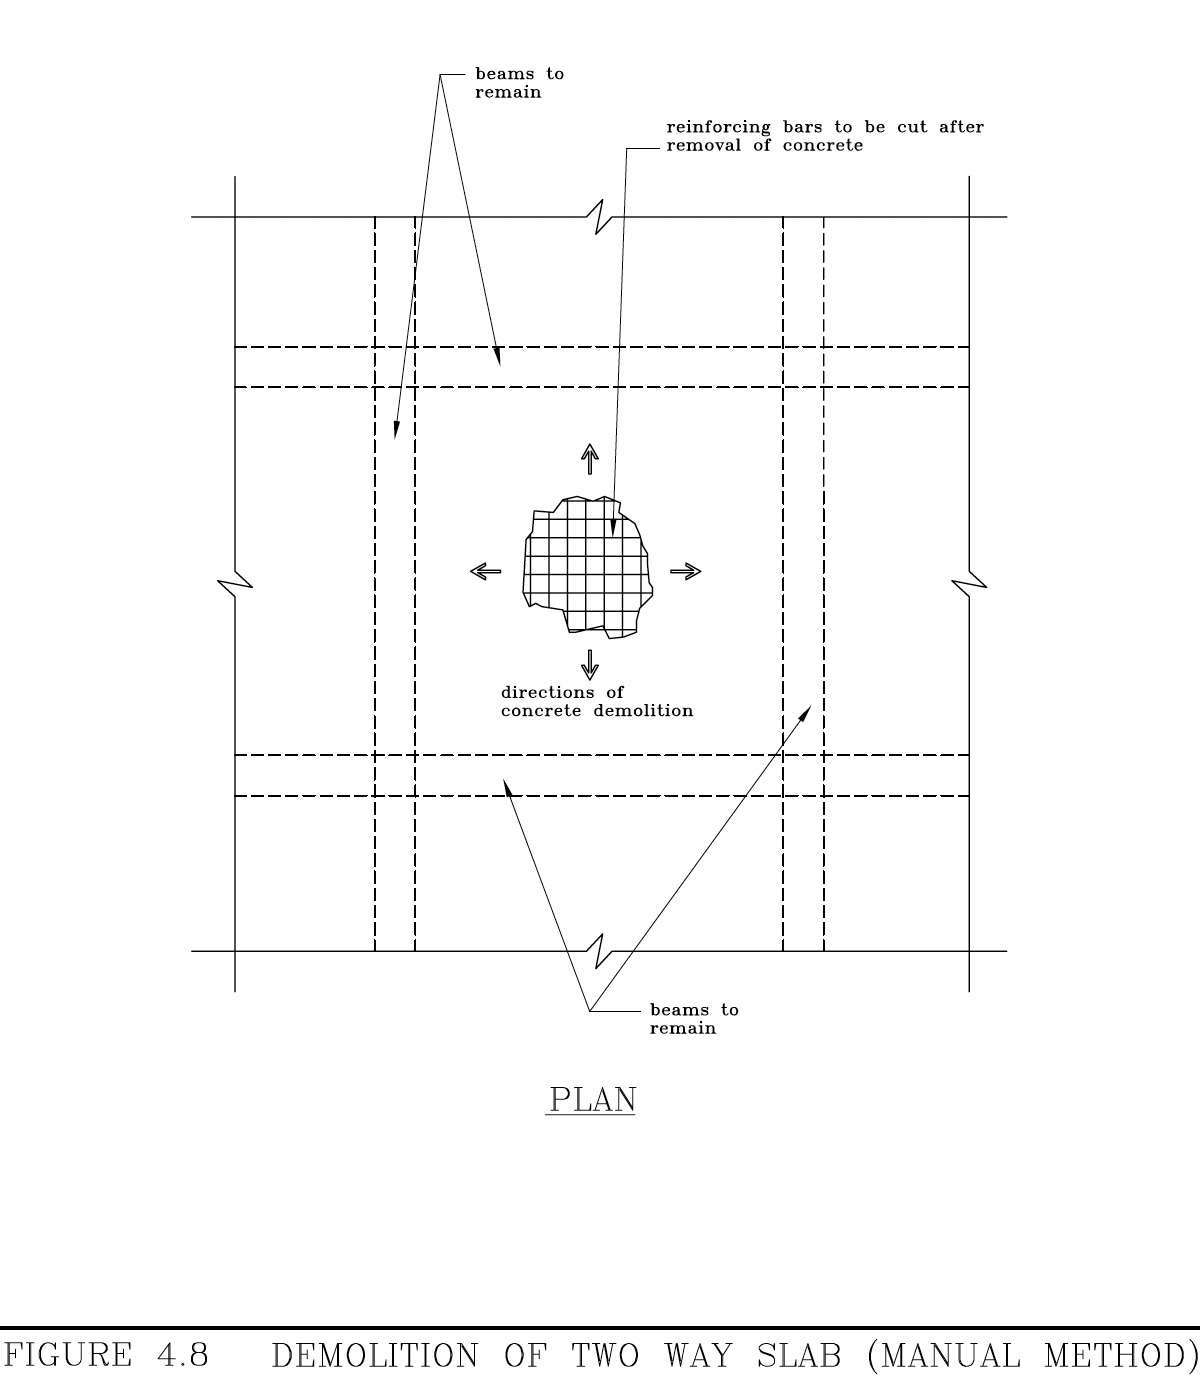
\includegraphics[width=0.5\textwidth]{figures/Demolition-of-Two-way-slab.jpeg}
    \caption{Regulation1}
    \label{fig:regulation1}
\end{figure}
Regulation2: 
\begin{figure}
    \centering
    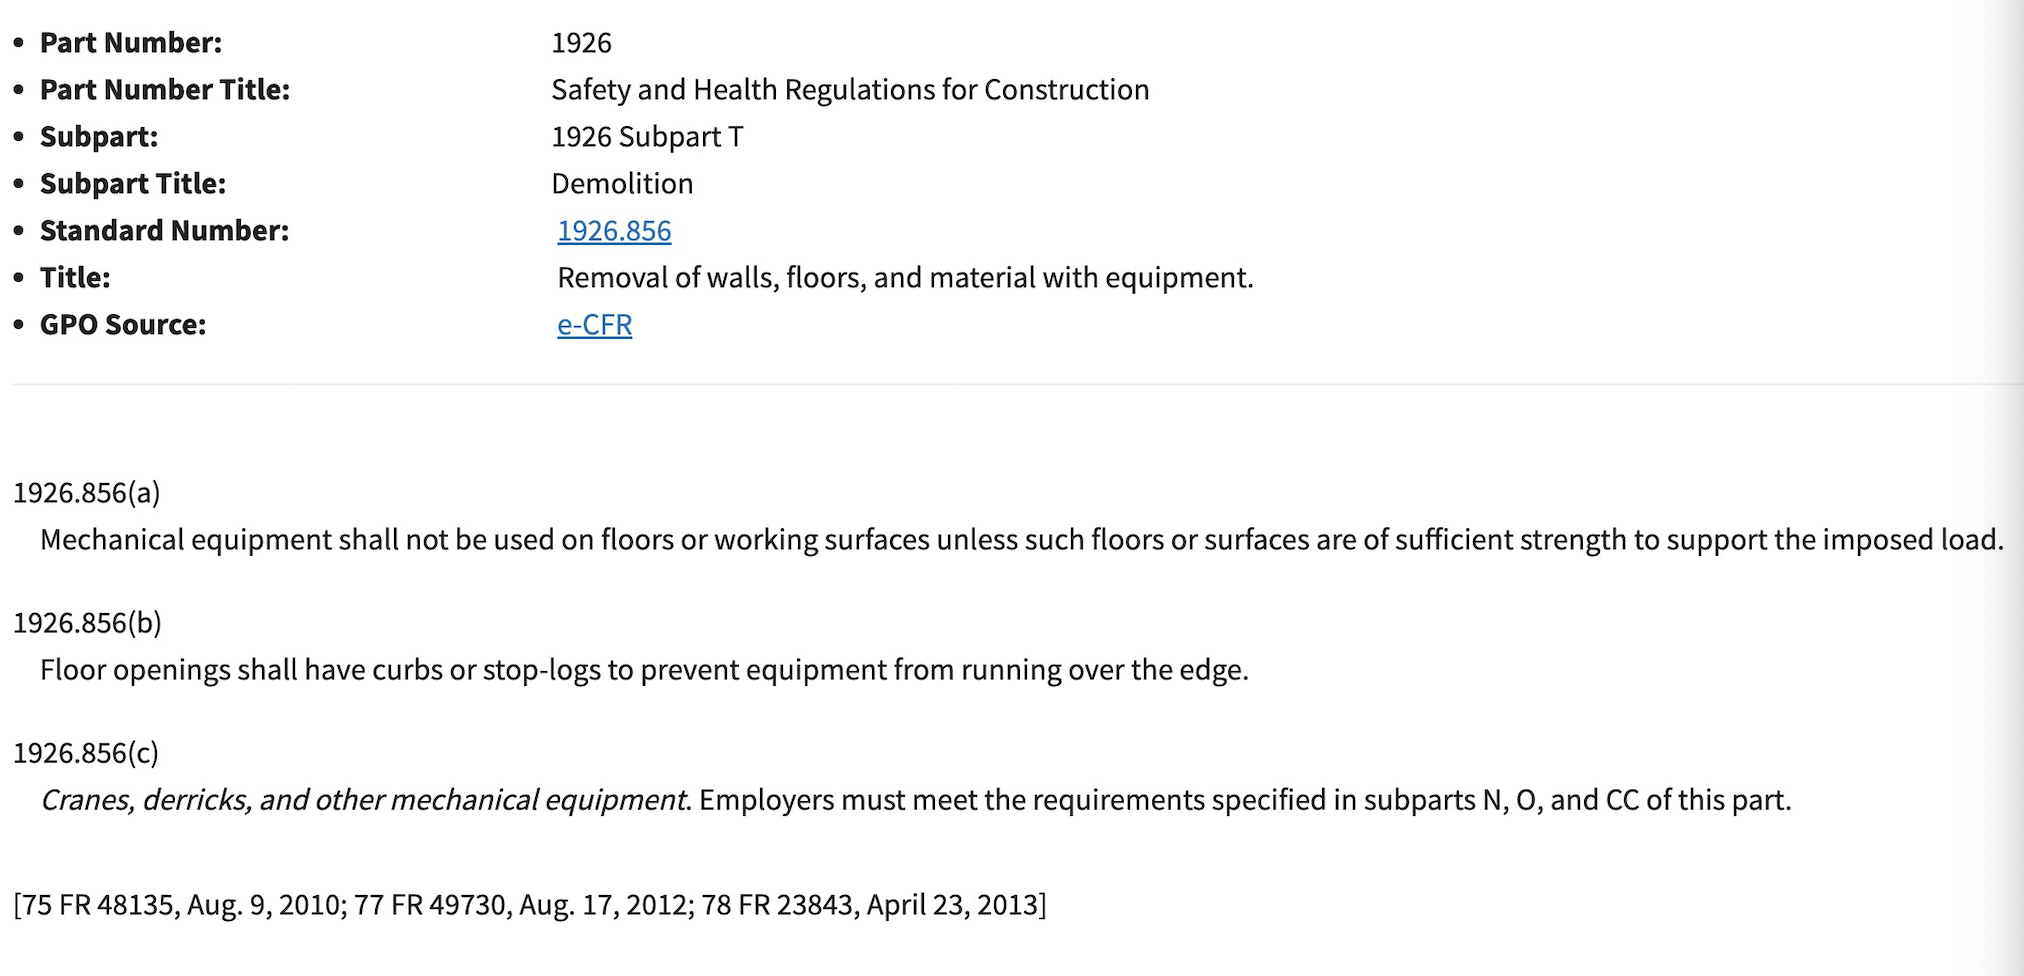
\includegraphics[width=0.5\textwidth]{figures/Removal-of-walls-floors-and-material-with-equipment.png}
    \caption{Regulation1}
    \label{fig:regulation1}
\end{figure}
Regulation3: 
\begin{figure}
    \centering
    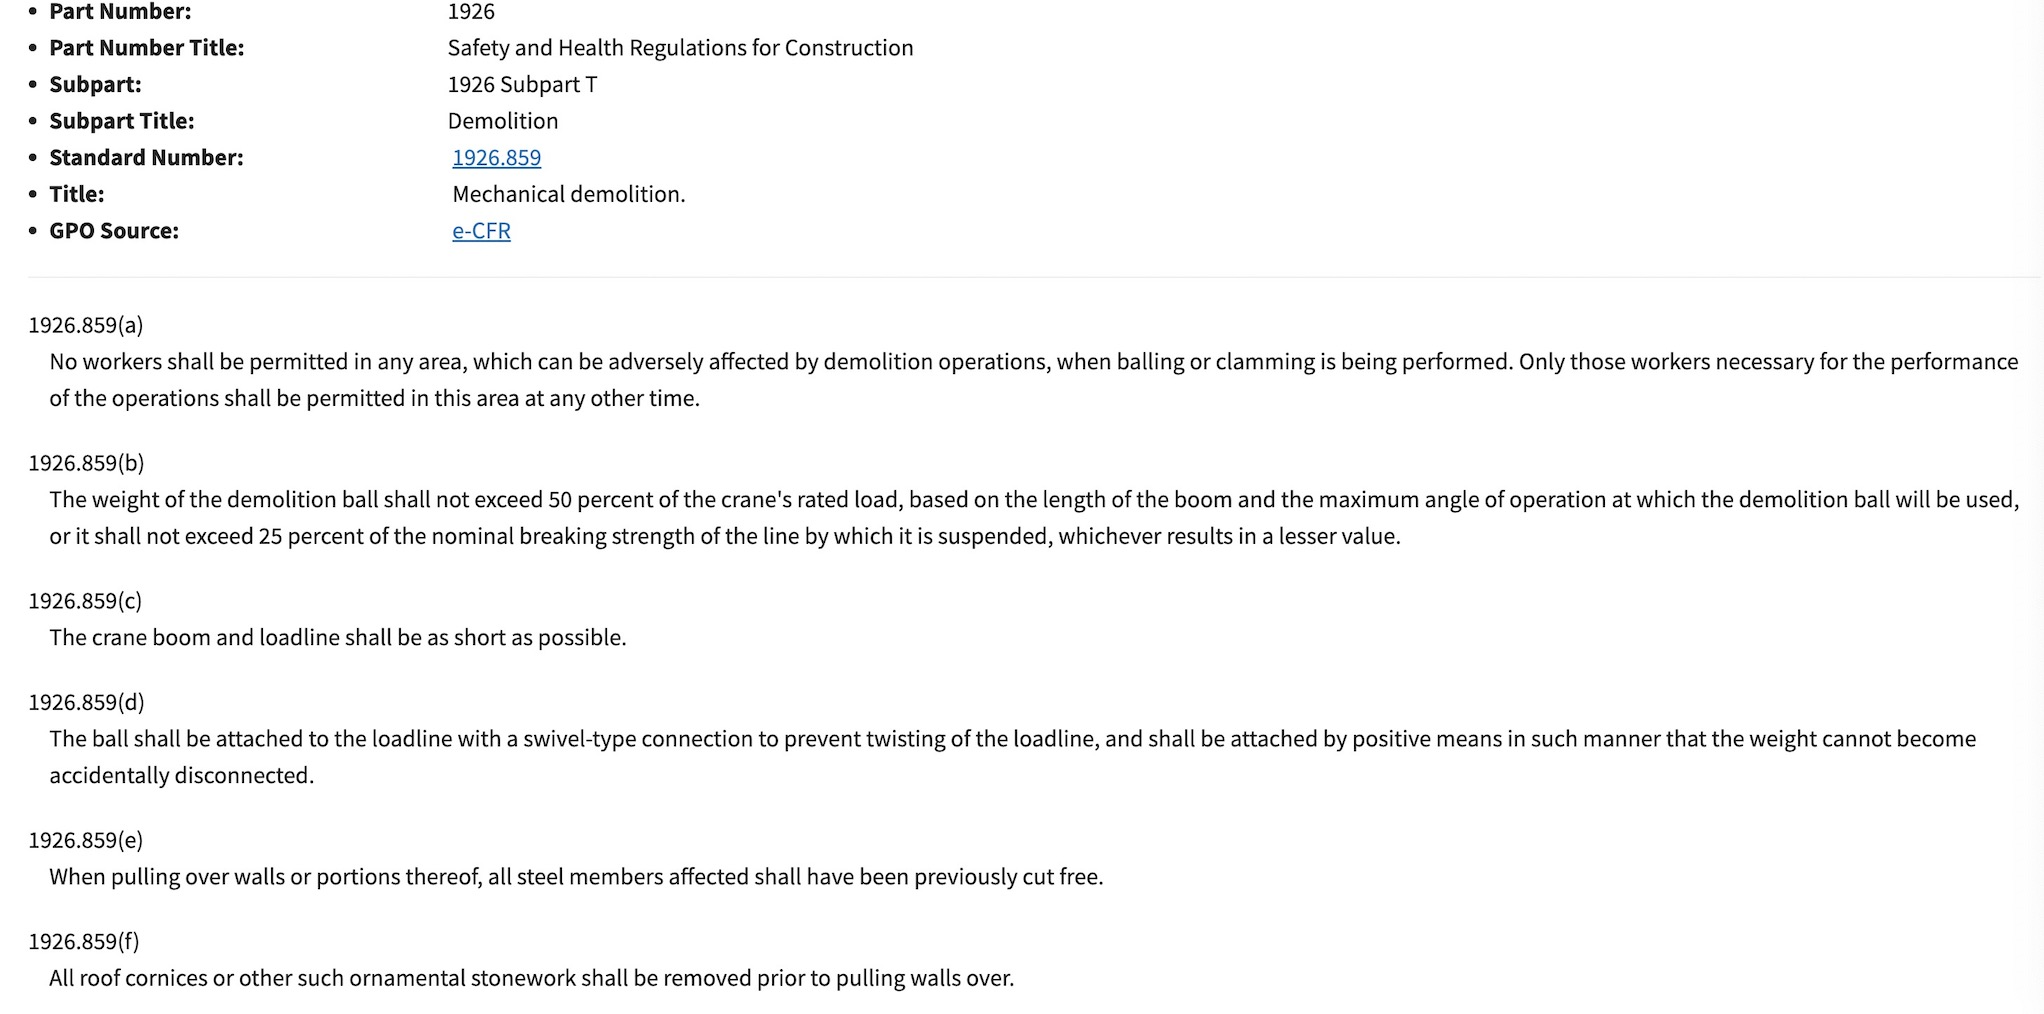
\includegraphics[width=0.5\textwidth]{figures/mechanical-demolition.jpeg}
    \caption{Regulation1}
    \label{fig:regulation1}
\end{figure}


\vspace{12pt}
\color{red}


\end{document}
